\documentclass[a4paper,fontsize=13pt]{scrreprt}

\usepackage[francais]{babel}

\usepackage[utf8]{inputenc}
\usepackage[T1]{fontenc}
\usepackage{pifont}
%\usepackage{verdana}
\usepackage{ulem}

\usepackage{amsmath}
\usepackage{amssymb}
\usepackage{amsthm}
\usepackage{amscd}
\usepackage{mathabx}
\usepackage{hyperref}
\usepackage{setspace} 
\usepackage{multicol}
\onehalfspacing

\usepackage[abbrev,backrefs]{amsrefs}
\usepackage{eurosym}

\usepackage{graphicx}
\usepackage{array}

\usepackage[framemethod=TikZ]{mdframed} % Cadres
\usepackage{tikz}
\usepackage{tkz-euclide}
\usetkzobj{all}
\usepackage{tikz-3dplot}
\usetikzlibrary{calc,backgrounds}

\usepackage[all]{xy}
\usepackage{flowchart}
\usetikzlibrary{arrows}

\usepackage{geometry}
\geometry{hmargin=2.5cm,vmargin=2.5cm}
\pagestyle{myheadings}
\renewcommand{\chaptermark}[1]{\markboth{\textbf{\thechapter. #1}}{}}
\renewcommand{\sectionmark}[1]{\markright{\textbf{\thesection. #1}}}

\renewcommand{\familydefault}{\sfdefault}

\theoremstyle{plain}
\newtheorem{thé}[subsection]{Théorème}
\newtheorem*{thé*}{Théorème}
\newtheorem{pro}[subsection]{Proposition}
\newtheorem*{pro*}{Proposition}
\newtheorem{cor}[subsection]{Corollaire}	
\newtheorem*{cor*}{Corollaire}
\newtheorem{lem}[subsection]{Lemme}		

\theoremstyle{definition}
\newtheorem{déf}[subsection]{Définition}
\newtheorem{exe}[subsection]{Exemple}
\newtheorem{con}[subsection]{Contre-exemple}
\newtheorem{rema}[subsection]{Remarque}	
\newtheorem*{rema*}{Remarque}	
\newtheorem*{nota}{Notation}
\newtheorem*{prob}{Problème}	
\newtheorem*{epcs}{Exercices pour cette section}
\newtheorem{exo}[subsection]{Exercice}
\newtheorem*{exo*}{Exercice}
\newtheorem*{solu}{Solution}

\newcommand{\nn}{\mathbb{N}}
\newcommand{\nno}{\mathbb{N}_{0}}
\newcommand{\zz}{\mathbb{Z}}
\newcommand{\qu}{\mathbb{Q}}
\newcommand{\rr}{\mathbb{R}}
\newcommand{\cc}{\mathbb{C}}
\newcommand{\imp}{\Rightarrow}

\DeclareMathOperator{\dom}{dom}
\DeclareMathOperator{\im}{im}

%---------------------------------------------------------------------------------------------------------------------------------
% Tikz
%---------------------------------------------------------------------------------------------------------------------------------

% Définition des nouvelles options xmin, xmax, ymin, ymax
\tikzset{
	xmin/.store in=\xmin, xmin/.default=-3, xmin=-3,
	xmax/.store in=\xmax, xmax/.default=3, xmax=3,
	ymin/.store in=\ymin, ymin/.default=-3, ymin=-3,
	ymax/.store in=\ymax, ymax/.default=3, ymax=3,
}

% Commande \grille qui trace la grille entre (xmin,ymin) et (xmax,ymax)
\newcommand {\grille}{\draw[help lines] (\xmin,\ymin) grid (\xmax,\ymax);}

% Commande \axes
\newcommand {\axes} {
	\draw[thick, ->] (\xmin,0) -- (\xmax+1,0);
	\draw[thick, ->] (0,\ymin) -- (0,\ymax+1);
	\draw (0,\ymax+0.5) node [left] {$y$};
	\draw (\xmax+0.5, 0) node [below] {$x$};
	\draw[thick] (-0.15,1)--(0.15,1) (1,-0.15)--(1,0.15);
	\draw (0,1)node[left]{$1$} (1,0)node[below]{$1$};
}

% Commande \axesnotick, axes sans les bâtonnets
\newcommand {\axesnotick} {
	\draw[thick, ->] (\xmin,0) -- (\xmax+1,0);
	\draw[thick, ->] (0,\ymin) -- (0,\ymax+1);
	\draw (0,\ymax+0.5) node [left] {$y$};
	\draw (\xmax+0.5, 0) node [below] {$x$};
}

% Commande qui limite l'affichage à (xmin,ymin) et (xmax,ymax)
\newcommand {\fenetre}{\clip (\xmin,\ymin) rectangle (\xmax,\ymax);}

% Bold enumerate
\newenvironment{benumerate}[1][0pt]{\begin{enumerate}\renewcommand{\makelabel}[1]{\textbf{##1}}\setlength{\itemsep}{#1}}{\end{enumerate}}
\renewcommand{\d}{\displaystyle}

\begin{document}
	
\begin{titlepage}
	
	\newcommand{\HRule}{\rule{\linewidth}{0.4mm}} % Defines a new command for the horizontal lines, change thickness here
	
	\center % Center everything on the page
	
	%----------------------------------------------------------------------------------------
	%	HEADING SECTIONS
	%----------------------------------------------------------------------------------------
	
	\vspace{4cm}
	
	\textsc{\Large Cours de mathématiques de cinquième année \\ 4 périodes/semaine \\ Année 2018-2019}\\[0.3cm]
	\vspace{9.4cm}
	\textsc{\LARGE Fonctions dérivables et dérivées}\\[0.6cm] % Major heading such as course name
	\vspace{9.8cm}
	\textsc{\Large Lycée Martin V}\\[0.3cm] % Minor heading such as course title
	

	
\end{titlepage}
	

\tableofcontents



\chapter{Introduction}

\section{Histoire et contexte} \label{Histoire et contexte}

Les historiens des sciences ont longtemps débattu au sujet de \og l'invention \fg{} des dérivées et du calcul différentiel et intégral en général : certains d'entre eux affirmaient que la première personne à avoir développé cette notion était Newton, le célèbre physicien qui a donné naissance à la physique classique moderne, tandis que d'autres affirmaient qu'il s'agit de Leibniz, un très grand philosophe et mathématicien contemporain de Newton. \\
Quoi qu'il en soit, ces idées ont été révolutionnaires : une majeure partie des sciences modernes n'existeraient pas sans les dérivées (et les intégrales\footnote{(que vous découvrirez en sixième année)}), de même pour de nombreuses technologies et techniques qui ont façonné notre société et nos modes de vie. \\
Par ailleurs, le calcul différentiel et intégral a un intérêt intrinsèque gigantesque : il fournit des outils aux mathématiciens d'une richesse qui semble inépuisable. Il s'agit véritablement d'un joyau de la connaissance humaine. \\
Même s'il est absurde d'affirmer que les dérivées sont nécessaires à une personne lambda pour vivre une vie ordinaire, toutes ces raisons font qu'on estime qu'il est souhaitable que ce sujet soit abordé dans un cours de mathématiques de secondaire et qu'une grande partie du cursus de mathématiques en secondaire est construit dans l'unique but d'aborder le calcul différentiel et intégral. \\
Malgré tout, les dérivées sont un sujet difficile et relativement technique. Avant d'introduire la définition fondamentale de fonction dérivable (en un point), nous allons donc nous intéresser à deux situations où l'idée de dérivée apparaît naturellement.

\section{Un peu de physique}

Dans le cours de physique de cinquième année secondaire, les mouvements rectilignes uniformes (MRU) et les mouvements rectilignes uniformément accélérés (MRUA) sont étudiés. \\
Un MRU consiste en le mouvement d'un corps (ponctuel) tel que ce mouvement se fasse dans une direction (et un sens) toujours identique et telle que la vitesse du corps soit constante (cette vitesse constante est notée $v_0$). Puisque la vitesse du corps est constante, le corps n'accélère pas et ne décélère pas. Puisque la vitesse du corps est contante, la distance entre le mobile et sa position initiale (dont l'éloignement avec un point de référence est noté $x_0$) est directement proportionnelle au temps $t$ écoulé depuis le début de l'observation du mouvement et le facteur de proportionnalité est $v_0$. Si on souhaite formaliser l'expression de la position du mobile (par rapport au point de référence) en fonction du temps, sa vitesse en fonction du temps et son accélération en fonction du temps, on a donc :
\begin{itemize}
	\begin{multicols}{3}
		\item [~] \begin{align*}
		x : [0;+\infty[ &\to \rr \\
		t &\mapsto x_0 + v_0 t
		\end{align*}
		\item [~] \begin{align*}
		v : [0;+\infty[ &\to \rr \\
		t &\mapsto v_0
		\end{align*}
		\item [~] \begin{align*}
		a : [0;+\infty[ &\to \rr \\
		t &\mapsto 0
		\end{align*}
	\end{multicols}
\end{itemize}
Ces trois formules, très utiles, sont également vues au cours de physique et sont utilisées pour résoudre de nombreux problèmes. Néanmoins, dans de nombreuses situations (la plus célèbre étant celle de la chute libre d'un corps à la surface terrestre lorsque les frottements de l'air sont négligés), le mouvement du mobile que l'on étudie ne correspond pas à un MRU, mouvement qui se fait donc dans une seule direction (et un seul sens) et dont la \textbf{vitesse} est constante, mais un MRUA, c'est-à-dire une mouvement qui se fait donc dans une seule direction (et un seul sens) mais dont l'\textbf{accélération} est constante et non nulle (une accélération négative correspond à une décélération ou à une accélération dans le sens opposé), notée $a_0$. Pour un tel type de mouvement, les formules suivantes sont données :
\begin{itemize}
	\begin{multicols}{3}
		\item [~] \begin{align*}
		x : [0;+\infty[ &\to \rr \\
		t &\mapsto x_0 + v_0 t + a_0 \frac{t^2}{2}
		\end{align*}
		\item [~] \begin{align*}
		v : [0;+\infty[ &\to \rr \\
		t &\mapsto v_0 + a_0 t
		\end{align*}
		\item [~] \begin{align*}
		a : [0;+\infty[ &\to \rr \\
		t &\mapsto a_0
		\end{align*}
	\end{multicols}
\end{itemize}
L'expression de la fonction exprimant l'accélération en fonction de la vitesse est évidente (l'accélération est constante et vaut toujours $a_0$). Celle de la vitesse n'est pas surprenante : puisque l'accélération du mobile est constante et non-nulle, la différence entre la vitesse du mobile à un moment $t$ et sa vitesse initiale est directement proportionnelle à $t$ et le facteur de proportionnalité est $a_0$. \\
Mais l'expression de la position du mobile en fonction du temps laisse perplexe, en particulier le terme $a_0 \frac{1}{2} t^2$ : d'où provient-il ? Pour essayer de le comprendre, réfléchissons d'abord sur ce que représentent vraiment les fonctions $x$, $v$ et $a$ et à ce qu'on entend précisément par vitesse (et accélération).
\begin{center}
	\begin{Large}
		Qu'est-ce que la vitesse ?
	\end{Large}
\end{center}
La notion de vitesse la plus élémentaire et la plus intuitive est celle de vitesse moyenne. Par exemple, si je parcours $800$km pour rejoindre la Provence pour mes vacances et que le trajet a duré $8$h, tout le monde s'accordera pour dire que ma vitesse \textbf{moyenne} pour ce trajet était de $\frac{800}{100}=100$km/h. De façon plus formelle, pour un mouvement d'un mobile effectué dans une unique direction où les positions du mobiles par rapport à un point de référence en fonction du temps sont notées $x_{(t)}$, la vitesse moyenne du mobile pour un intervalle de temps $[t_1 ; t_2]$ est $\frac{x_{(t_2)} - x_{(t_1)}}{t_2 - t_1}$, ce que certains physiciens notent de façon abrégée $\frac{\Delta x}{\Delta t}$. \\
Néanmoins, il nous arrive également de parler de la vitesse d'un mobile à un certain instant $t$ bien précis. Par exemple, certaines voitures ont un compteur qui affiche ce que la plupart des gens considèrent être la vitesse de la voiture à chaque instant, vitesse qui évolue donc de façon continue au cours du temps et n'est pas constante. Dans ce cas, on parle de vitesse \textbf{instantannée} et non de vitesse moyenne : on souhaite exprimer l'idée que la voiture roule à une certaine vitesse précise à un moment précis (et non une moyenne sur un intervalle de temps choisi). Mais quelle est la définition de la vitesse instantannée (qui est donc celle utilisée dans les formules du MRU et du MRUA listées ci-dessus) et comment la calcule-t-on ? \\
Pour construire la défintion de vitesse instantannée, peut-être pouvons-nous nous aider de la notion de vitesse moyenne (et de sa définition). Plaçons nous donc à nouveau dans le cadre formel suivant : on considère un mouvement d'un mobile réalisé dans une unique direction où les positions du mobile par rapport à un point de référence en fonction du temps sont notées $x_{(t)}$. Puisque nous souhaitons définir l'idée de vitesse instantannée, à un moment $t_1$ bien précis, pourquoi ne pas reprendre la définition de la vitesse moyenne mais imposer que l'intervalle de temps considéré doit avoir une durée nulle, autrement dit que $t_1 = t_2$ ? \\
Malheureusement, cette approche intuitive pour définir la vitesse instantannée a un problème. En effet, si $t_1 = t_2$, la formule $\frac{x_{(t_2)} - x_{(t_1)}}{t_2 - t_1}$ ne fait pas sens (car on divise par $0$) ! Allons-nous donc devoir développer une toute approche pour définir rigoureusement (et être capable de calculer) une vitesse instantannée ? Heureusement, non. \\
Même si la formule $\frac{x_{(t_2)} - x_{(t_1)}}{t_2 - t_1}$ ne fait pas sens si $t_1 = t_2$, il fait bien sens de se demander de quoi se rapproche cette quantité au fur et à mesure que l'intervalle de temps devient de plus en plus petit, autrement dit au fur et à mesure que $t_2$ se rapproche de $t_1$. Or, nous avons à présent un outil mathématique qui nous permet de formaliser cette idée (et calculer) : celle de limite ! Dès lors, nous pouvons définir la vitesste instantannée à un moment $t_1$ comme étant la valeur $$\lim\limits_{t_2 \to t_1} \frac{x_{(t_2)} - x_{(t_1)}}{t_2 - t_1}$$
à condition que cette limite existe, bien entendu. \\
Fantastique : si nous choisissons cette définition pour la vitesse instantannée\footnote{Et il s'agit justement de la définition choisie par tous les physiciens du monde. \c{C}a tombe bien.}, il nous suffit d'être capable de déterminer quand la limite $\lim\limits_{t_2 \to t_1} \frac{x_{(t_2)} - x_{(t_1)}}{t_2 - t_1}$ existe et comment la calculer dans ce cas pour comprendre le lien entre les différentes formules du MRUA. \\
Cette limite est une limite particulière : c'est la limite d'un quotient différentiel spécifique. Ce type de limite porte un nom : il s'agit en fait d'une dérivée. Comprendre les formules du MRUA et apprendre à calculer une vitesse instantannée constituent donc nos premières raisons d'étudier en détail ces limites particulières (les dérivées). Dans les prochaines sections, nous les étudierons pour elles-mêmes et nous reviendrons ensuite sur ce petit voyage du côté de la physique.

\section{Un vieux problème d'optimisation}

Lorsqu'il a fallu se décider il y a plus d'un siècle sur la meilleure forme pour les boites de conserves et les canettes, tout le monde s'est rapidement mis d'accord : le cylindre est très pratique. Des boites de conserves cylindriques peuvent être empilées, rangées côte à côte sans trop perdre d'espace, peuvent être prises en main sans risque de se blesser et peuvent être déplacées facilement en les faisant rouler. Que demander de plus ?\\
Néanmoins, le consensus n'était pas parfait. Il restait à se décider sur le type de cylindre : plutôt long, plutôt plat ?

\begin{itemize}
	\begin{multicols}{3}
		\item [~] \begin{tikzpicture}[scale=0.5]
		\draw (0,0) ellipse (1cm and 0.5cm);
		\draw (-01,0) -- (-1,-8);
		\draw (1,0) -- (1,-8);
		\draw (0,-8) ellipse (1cm and 0.5cm);
		\end{tikzpicture}
		\item [~] \begin{tikzpicture}[scale=0.5]
		\draw (0,0) ellipse (2cm and 1cm);
		\draw (-2,0) -- (-2,-5);
		\draw (2,0) -- (2,-5);
		\draw (0,-5) ellipse (2cm and 1cm);
		\end{tikzpicture}
		\item [~] \begin{tikzpicture}[scale=0.5]
		\draw (0,0) ellipse (4cm and 2cm);
		\draw (-4,0) -- (-4,-2);
		\draw (4,0) -- (4,-2);
		\draw (0,-2) ellipse (4cm and 2cm);
		\end{tikzpicture}
	\end{multicols}
\end{itemize}

Afin de minimiser la quantité de matériau utilisée pour fabriquer chaque conserve/canette, le cylindre à privilégier est celui qui minimise l'aire de la surface externe. On a donc dû déterminer quelles étaient les dimensions optimales d'un cylindre de volume donné, c'est-à-dire celles qui minimisent sa surface. Nous allons essayer de trouver nous-même ces dimensions dans le cas d'une canette d'un volume de $330$ml, c'est-à-dire de $330$cm$^3$. \\
Nous avons donc deux paramètres variables, la hauteur de la canette (notée $h$) et son rayon (noté $r$) :
\begin{center}
	\begin{tikzpicture}[scale=1]
	\draw[dashed,color=gray] (0,0) ellipse (2cm and 1cm);
	\draw  (0,0) -- (2,0);
	\draw (1,0.3) node {$r$};
	\draw[dashed,color=gray] (-2,0) -- (-2,-5);
	\draw[dashed,color=gray] (2,0) -- (2,-5);
	\draw  (0,0) -- (0,-5);
	\draw (0.3,-2.5) node {$h$};
	\draw[dashed,color=gray] (0,-5) ellipse (2cm and 1cm);
	\end{tikzpicture}
\end{center}
Tout d'abord, puisque le volume de la canette que l'on souhaite fabriquer doit être de $330$cm$^3$, notons que plus le rayon de la canette sera grand, plus sa hauteur devra être petite et inversément. En fait, nous pouvons même être plus précis : puisque le volume d'un cylindre de rayon $r$ et de hauteur $h$ est $\pi r^2 h$ (l'aire de la base, $\pi r^2$, fois la hauteur $h$), on a l'équation :
$$330=\pi r^2 h$$
Ou encore :
$$h=\frac{330}{\pi r^2}$$
Par ailleurs, l'aire de la surface d'un cylindre de rayon $r$ et de hauteur $h$ est égale à la somme des aires du disque du dessus, c'est-à-dire $\pi r^2$, du disque du dessous, c'est-à-dire à nouveau $\pi r^2$, et de l'aire de la surface latérale qui est égale à $2\pi r h$ (la longueur du périmètre de la base, c'est-à-dire $2\pi r$, fois la hauteur $h$), ce qui nous donne :
$$\pi r^2+\pi r^2+2\pi r h=2\pi r^2+2\pi r h$$
Nous pouvons substituer le lien entre $h$ et $r$ obtenu ci-dessus afin d'obtenir une fonction nous donnant l'aire de la surface extérieure d'une canette cylindrique dont le volume est $330$cm$^3$ en fonction de son rayon $r$ :
\begin{align*}
A : ]0;+\infty[ &\to \rr \\
r \mapsto& 2\pi r^2+ \frac{660}{r}
\end{align*}
Nous devons donc trouver la valeur de $r$ qui minimise cette fonction. À cette fin, réalisons le graphe de cette fonction (en injectant quelques valeurs dans son expression) :
\begin{center}
	\begin{tikzpicture}[domain=0.82:8] 
	\draw[very thin,color=gray] (-0.1,-0.1) grid (7.9,7.9);
	\draw[->] (-0.2,0) -- (8.2,0) node[right] {$r$ (cm)}; 
	\draw[->] (0,-0.2) -- (0,8.2) node[above] {$A(r)$ (cm$^2$)};
	\draw (1,-0.2) node[below] {$1$}; 
	\draw (-0.2,1) node[left] {$100$}; 
	\draw[thick] plot (\x,\x * \x *0.01*2*3.14159+6.6*1/\x);
	\end{tikzpicture}
\end{center}
Cette fonction semble avoir un point de minimum entre $3$ et $4$, mais comment déterminer précisément celui-ci ?
Si nous prenons deux points du graphe, $(r_1;A(r_1))$ et $(r_2;A(r_2))$, nous pouvons calculer la pente de la droite passant par ces deux points : $\frac{A(r_2)-A(r_1)}{r_2 - r_1}$.
Supposons que pour chaque point du graphe $(r_1;A(r_1))$, nous parvenions à déterminer la pente de la droite qui passe par ce point et ce point uniquement : elle \og frôle \fg{} le graphe de la fonction et ne le touche qu'en un seul point, le point $(r_1;A(r_1))$\footnote{Plus tard, nous définirons clairement et rigoureusement cette notion, que l'on nomme tangente.}. Intuitivement, il suffirait alors de déterminer le point $(r_1;A(r_1))$ où la pente de cette droite est nulle pour trouver celui où on est au plus bas (pensez à l'inclinaison d'une voiture en montagne : elle sera \og à plat \fg{} soit lorsqu'elle se trouve au sommet d'une montagne/colline, soit lorsqu'elle se trouve au fond de la vallée), ce qui nous permettrait de trouver le rayon le plus avantageux et donc de résoudre notre problème d'optimisation.
Mais comment calculer la pente d'une telle droite ? Si on se base sur notre intuition, celle-ci devrait avoir comme pente le nombre dont se rapproche les pentes des droites passant par le point $(r_1;A(r_1))$ fixé et un point $(r_2;A(r_2))$ variable. Autrement dit, la pente de ce qu'on nommera plus tard la tangente au graphe de la fonction $A$ au point $(r_2;A(r_2))$ devrait être égale à :
$$\lim\limits_{r_2 \to r_1}\frac{A(r_2)-A(r_1)}{r_2 - r_1}$$
On retrouve une fois de plus cette limite d'un quotient différentiel spécifique. Bref, une étude approdfondie de ce type de limite semble inévitable : c'est ce que nous allons commencer à faire dans la prochaine section.

\chapter{Définition et exemples}

Voici la définition fondamentale de ce chapitre :
\begin{déf}
	Soit $I = ]a,b[$ un intervalle. Soit $c \in I$. Soit $f : I \to \rr$. \\On dit que $f$ est \emph{dérivable} en $c$ si et seulement si la \emph{fonction d'accroissement} de $f$ en $c$, c'est-à-dire la fonction
	\begin{align*}
	A_{f;c} : I \backslash \{c\} &\to \rr \\
	x &\mapsto \frac{f(x)-f(c)}{x-c}
	\end{align*}
	a une limite en $c$, c'est-à-dire si et seulement si la limite
	$$\lim\limits_{x\to c} \frac{f(x)-f(c)}{x-c}$$
	existe. \\
	Dans ce cas, on note $f'(c)$ la limite $\lim\limits_{x\to c} \frac{f(x)-f(c)}{x-c}$ qu'on nomme \emph{nombre dérivé} de $f$ en $c$.
\end{déf}
\begin{rema}
	À nouveau, la définition est donnée ici dans un cadre simple mais peut faire sens dans un cadre beaucoup plus général.
\end{rema}
Avant toute autre chose :
\begin{pro}
	Soit $I = ]a,b[$ un intervalle. Soit $c \in I$. Soit $f : I \to \rr$. \\
	Alors : si $f$ est dérivable en $c$, le nombre dérivé de $f$ en $c$ est unique.
\end{pro}
\begin{proof}
	La démonstration est directe puisque si une fonction a une limite en un point, cette limite est unique (voir chapitre(s) sur les limites (de fonctions)).
\end{proof}
\begin{rema}
	La proposition précédente permet de s'assurer qu'il fait bien sens de parler \textbf{du} nombre dérivé en un point.
\end{rema}
Donnons à présent quelques exemples.
\begin{exe}
	La fonction constante de constante $2$ est-elle dérivable en $3$ ? \\
	Cette question revient à se demander si la limite
	$$\lim\limits_{x\to 3} \frac{f(x)-f(3)}{x-3}$$
	existe, où $f$ est la fonction
	\begin{align*}
	f : \rr &\to \rr \\
	x &\mapsto 2
	\end{align*}
	Pour le déterminer, remarquons d'abord que pour tout $x \in \rr \backslash \{3\}$, on a :
	$$\frac{f(x)-f(3)}{x-3} = \frac{2-2}{x-3} = \frac{0}{x-3} = 0$$
	Dès lors :
	$$\lim\limits_{x\to 3} \frac{f(x)-f(3)}{x-3} = \lim\limits_{x\to 3} 0=0$$
	Donc la limite $\lim\limits_{x\to 3} \frac{f(x)-f(3)}{x-3}$ existe et le nombre dérivé en $3$ de la fonction constante de constante $2$ est égal à $0$ : $f'(3)=0$.
\end{exe}
\begin{exe}
	La fonction identité est-elle dérivable en $-5$ ? \\
	Cette question revient à se demander si la limite
	$$\lim\limits_{x\to -5} \frac{f(x)-f(-5)}{x-(-5)}$$
	existe, où $f$ est la fonction
	\begin{align*}
	f : \rr &\to \rr \\
	x &\mapsto x
	\end{align*}
	Pour le déterminer, remarquons d'abord que pour tout $x \in \rr \backslash \{-5\}$, on a :
	$$\frac{f(x)-f(-5)}{x-(-5)} = \frac{x+(-5)}{x+5} = \frac{x+5}{x+5} = 1$$
	Dès lors :
	$$\lim\limits_{x\to -5} \frac{f(x)-f(-5)}{x-(-5)} = \lim\limits_{x\to -5} 1=1$$
	Donc la limite $\lim\limits_{x\to -5} \frac{f(x)-f(-5)}{x-(-5)}$ existe et le nombre dérivé en $-5$ de la fonction identité est égal à $1$ : $f'(-5)=1$.
\end{exe}
\begin{exe}
	La fonction carrée est-elle dérivable en $1$ ? \\
	Cette question revient à se demander si la limite
	$$\lim\limits_{x\to 1} \frac{f(x)-f(1)}{x-1}$$
	existe, où $f$ est la fonction
	\begin{align*}
	f : \rr &\to \rr \\
	x &\mapsto x^2
	\end{align*}
	Pour le déterminer, remarquons d'abord que pour tout $x \in \rr \backslash \{1\}$, on a :
	$$\frac{f(x)-f(1)}{x-1} = \frac{x^2-1^2}{x-1} = \frac{(x+1)(x-1)}{x-1} = x+1$$
	Dès lors, puisque la fonction définie sur $\rr$ qui associe à tout nombre réel $x$ le nombre $x+1$ est continue en $1$ :
	$$\lim\limits_{x\to 1} \frac{f(x)-f(1)}{x-1}= \lim\limits_{x\to 1} x+1=1+1=2$$
	Donc la limite $\lim\limits_{x\to 1} \frac{f(x)-f(1)}{x-1}$ existe et le nombre dérivé en $1$ de la fonction identité est égal à $2$ : $f'(1)=2$.
\end{exe}
\begin{con}
	La fonction valeur absolue est-elle dérivable en $0$ ? \\
	Cette question revient à se demander si la limite
	$$\lim\limits_{x\to 0} \frac{f(x)-f(0)}{x-0}$$
	existe, où $f$ est la fonction
	\begin{align*}
	f : \rr &\to \rr \\
	x &\mapsto |x|
	\end{align*}
	Pour le déterminer, remarquons d'abord que pour tout $x \in \rr \backslash \{0\}$, on a :
	$$\frac{f(x)-f(0)}{x-0} = \frac{|x|-0}{x-0} = \frac{|x|}{x}$$
	Dès lors, la limite $\lim\limits_{x\to 0} \frac{f(x)-f(0)}{x-0}$ existe si la limite $\lim\limits_{x\to 0} \frac{|x|}{x}$ existe. Réalisons le graphe de la fonction
	\begin{align*}
	f : {\rr}_0 &\to \rr \\
	x &\mapsto \frac{|x|}{x}
	\end{align*}
	pour nous aider à répondre à cette question (en injectant quelques valeurs dans l'expression de la fonction) :
	\begin{center}
		\begin{tikzpicture}[xmin=-5,xmax=5,ymin=-5,ymax=5,scale=0.6]{\grille\axes}
		\draw[very thick,color=blue] plot[domain=-5:0](\x,{-1});
		\draw[very thick,color=blue] plot[domain=0:5](\x,{1});
		\draw[thick, fill=white](0,1)circle(0.2);
		\draw[thick, fill=white](0,-1)circle(0.2);
		\end{tikzpicture}
	\end{center}
Clairement, cette fonction n'a pas de limite en $0$ (lorsque les $x$ se rapprochent de $0$, les $f(x)$ ne se rapprochent pas uniformément d'une unique valeur). Autrement dit, la limite $\lim\limits_{x\to 0} \frac{|x|}{x}$ n'existe pas. \\
	En conclusion : la fonction valeur absolue n'est pas dérivable en $0$.
\end{con}
Tous ces exemples nous montrent que déterminer si une fonction est dérivable en un point (et calculer son nombre dérivé en ce point s'il existe) peut être parfois un peu long, un peu calculatoire, voire même potentiellement difficile. Si nous désirons pouvoir utiliser cette notion de façon efficace, il nous faudra trouver un moyen de répondre à ce type de question plus rapidement. Pour ce faire, à l'instar de la façon dont nous avions procédé pour les fonctions continues, nous allons nous intéresser à la dérivabilité des fonctions de références avant de nous intéresser à la façon dont se combinent deux fonctions dérivables en un point. C'est à quoi nous allons nous atteler dans les deux prochaines sections. \\
~~\\
Avant de clore cette section, une dernière définition :
\begin{déf}
	Soit $I = ]a,b[$ un intervalle. Soit $f : I \to \rr$. \\On dit que $f$ est \emph{dérivable} (partout) si elle est dérivable en tout point $c \in I$. \\Dans ce cas, on note $f'$ la \emph{dérivée} de $f$, c'est-à-dire la fonction définie sur $\dom(f)$ qui associe à tout $x \in \dom(f)$ le nombre dérivé de $f$ en $x$ :
	\begin{align*}
	f' : I &\to \rr \\
	x &\mapsto f'(x)
	\end{align*}
\end{déf}

\begin{exo} \label{exodef}
	À partir de la définition de fonction dérivable (uniquement), déterminer si...
	\begin{enumerate}
		\item La fonction inverse est dérivable en $2$.
		\item La fonction cubique est dérivable en $-8$.
		\item La fonction valeur absolue est dérivable en $-\frac{3}{2}$.
		\item La fonction racine cubique est dérivable en $0$.
		\item La fonction racine carrée est dérivable en $16$.
		\item La fonction racine carrée est dérivable en $0$.
	\end{enumerate}
\end{exo}
%OB
%\begin{solu}
%	\begin{enumerate}
%		\item Oui. La question revient à savoir si la limite $$\lim\limits_{x \to 2} \frac{\frac{1}{x}-\frac{1}{2}}{x-2}$$ existe. \\
%		Or, pour tout $x \in \rr \backslash \{0,2\}$, on a $\frac{\frac{1}{x}-\frac{1}{2}}{x-2} = \frac{\frac{2-x}{2x}}{x-2}
% =\frac{-1}{2x}$. \\
% Dès lors, puisque la fonction définie sur ${\rr}_0$ qui associe à tout nombre réel $x$ non nul le nombre $\frac{-1}{2x}$ est continue en $2$ : $$\lim\limits_{x \to 2} \frac{\frac{1}{x}-\frac{1}{2}}{x-2} = \lim\limits_{x \to 2} \frac{-1}{2x} = \frac{-1}{2.2}=\frac{-1}{4}$$
% En conclusion, la fonction inverse est bien dérivable en $2$ et son nombre dérivé en $2$ est $\frac{-1}{4}$.
% 		\item Oui. Son nombre dérivé en $-8$ est $192$.
%		\item Oui. Son nombre dérivé en $-\frac{3}{2}$ est $-1$.
%		\item Non.
%		\item Oui. Son nombre dérivé en $16$ est $\frac{1}{8}$.
%		\item Non.
%	\end{enumerate}
%\end{solu}

\chapter{Dérivabilité des fonctions de références}
Commençons par la fonction de référence la plus simple, la fonction constante.
\begin{pro}
	La fonction constante de constante $k \in \rr$ est dérivable et sa dérivée vaut $0$ en tout point.
\end{pro}
\begin{proof}
	Montrons que la fonction
	\begin{align*}
	f : \rr &\to \rr \\
	x &\mapsto k
	\end{align*}
	est dérivable en un point $c \in \rr$ quelconque, autrement dit que la limite
	$$\lim\limits_{x \to c} \frac{f(x)-f(c)}{x-c}$$
	existe. \\
	Notons que pour tout $x \in \rr \backslash \{c\}$, on a :
	$$\frac{f(x)-f(c)}{x-c} = \frac{k-k}{x-c} = \frac{0}{x-c} = 0$$
	Dès lors :
	$$\lim\limits_{x \to c} \frac{f(x)-f(c)}{x-c} = \lim\limits_{x \to c} 0 = 0$$
	Quelle que soit la valeur de $c$, $f$ est donc bien dérivable en $c$ et on a $f'(c)=0$.
\end{proof}
À présent, une autre fonction de référence simple : la fonction identité.
\begin{pro}
	La fonction identité est dérivable et sa dérivée vaut $1$ en tout point.
\end{pro}
\begin{proof}
	Montrons que la fonction
	\begin{align*}
	f : \rr &\to \rr \\
	x &\mapsto x
	\end{align*}
	est dérivable en un point $c \in \rr$ quelconque, autrement dit que la limite
	$$\lim\limits_{x \to c} \frac{f(x)-f(c)}{x-c}$$
	existe. \\
	Notons que pour tout $x \in \rr \backslash \{c\}$, on a :
	$$\frac{f(x)-f(c)}{x-c} = \frac{x-c}{x-c} = 1$$
	Dès lors :
	$$\lim\limits_{x \to c} \frac{f(x)-f(c)}{x-c} = \lim\limits_{x \to c} 1 = 1$$
	Quelle que soit la valeur de $c$, $f$ est donc bien dérivable en $c$ et on a $f'(c)=1$.
\end{proof}
La dernière fonction de référence pour laquelle nous ferons la démonstration de sa dérivabilité est la fonction carrée.
\begin{pro}
	La fonction carrée est dérivable et $\forall c \in \rr$, sa dérivée vaut $2c$ en $c$.
\end{pro}
\begin{proof}
	Montrons que la fonction
	\begin{align*}
	f : \rr &\to \rr \\
	x &\mapsto x^2
	\end{align*}
	est dérivable en un point $c \in \rr$ quelconque, autrement dit que la limite
	$$\lim\limits_{x \to c} \frac{f(x)-f(c)}{x-c}$$
	existe. \\
	Notons que pour tout $x \in \rr \backslash \{c\}$, on a :
	$$\frac{f(x)-f(c)}{x-c} = \frac{x^2-c^2}{x-c} = \frac{(x-c)(x+c)}{x-c} = x+c$$
	Dès lors, puisque la fonction
	\begin{align*}
	g : \rr &\to \rr \\
	x &\mapsto x+c
	\end{align*}
	est continue en $c$ :
	$$\lim\limits_{x \to c} \frac{f(x)-f(c)}{x-c} = \lim\limits_{x \to c} x+c = 2c$$
	Quelle que soit la valeur de $c$, $f$ est donc bien dérivable en $c$ et on a $f'(c)=2c$.
\end{proof}
La démonstration de la dérivabilité de la fonction carrée peut facilement être généralisée pour démontrer la dérivabilité de la fonction puissance où l'exposant est un nombre naturel non nul :
\begin{pro}
	Soit $n \in \nn \backslash \{0\}$. La fonction
	\begin{align*}
	f : \rr &\to \rr \\
	x &\mapsto x^n
	\end{align*}
	est dérivable et $\forall c \in \rr$, on a $f'(c) = nc^{n-1}$.
\end{pro}
\begin{proof}
	Pas en math $4$.
\end{proof}
\begin{rema}
	Si on prend $n =3$ dans la proposition précédente, on retrouve par exemple la fonction cubique :
	\begin{align*}
	f : \rr &\to \rr \\
	x &\mapsto x^3
	\end{align*}
	Cette fonction est donc dérivable et sa dérivée vaut $f'(x)=3x^2$.
\end{rema}
La proposition précédente peut être généralisée au cas où l'exposant de la fonction puissance peut être un nombre entier non nul, mais le domaine doit être réduit.
\begin{pro}
	Soit $n \in \zz \backslash \{0\}$. La fonction
	\begin{align*}
	f : {\rr}_{0} &\to \rr \\
	x &\mapsto x^n
	\end{align*}
	est dérivable et $\forall c \in \rr$, on a $f'(c) = nc^{n-1}$.
\end{pro}
\begin{proof}
	Pas en math $4$.
\end{proof}
\begin{rema}
	Si on prend $n =-1$ dans la proposition précédente, on retrouve par exemple la fonction inverse\footnote{Rappel : pour tout $x \in \rr \backslash \{0\}$, on a $x^{-1}=\frac{1}{x}$.} :
	\begin{align*}
	f : \rr &\to \rr \\
	x &\mapsto \frac{1}{x}
	\end{align*}
	Cette fonction est donc dérivable et sa dérivée vaut $f'(x)=-x^{-2}=\frac{-1}{x^2}$.
\end{rema}
On peut encore généraliser au cas où l'exposant de la fonction puissance peut être un nombre rationnel non nul, mais le domaine doit être encore réduit.
\begin{pro}
	Soit $n \in \qu \backslash \{0\}$. La fonction
	\begin{align*}
	f : {\rr}^{+}_{0} &\to \rr \\
	x &\mapsto x^n
	\end{align*}
	est dérivable et $\forall c \in \rr$, on a $f'(c) = nc^{n-1}$.
\end{pro}
\begin{proof}
	Pas en math $4$.
\end{proof}
\begin{rema}
	Si on prend $n =\frac{1}{2}$ dans la proposition précédente, on retrouve par exemple la fonction racine carée\footnote{Rappel : pour tout $x \in \rr \backslash \{0\}$, on a $x^{\frac{1}{2}}=\sqrt{x}$.} réduite sur ${\rr}^{+}_{0}$ :
	\begin{align*}
	f : {\rr}^{+}_{0} &\to \rr \\
	x &\mapsto \sqrt{x}
	\end{align*}
	Cette fonction est donc dérivable et sa dérivée vaut $f'(x)=\frac{1}{2}x^{-\frac{1}{2}}=\frac{1}{2\sqrt{x}}$. \\
\end{rema}
La proposition précédente ne nous dit donc pas si les fonctions racine carrée et racine cubique sont dérivables en $0$. Elles ne le sont pas : voir exercice \ref{exodef}. \\
~~\\
Il ne nous reste plus qu'à traiter le cas de la fonction valeur absolue.
\begin{pro}
	La fonction valeur absolue est dérivable en tout point $c \in {\rr}_{0}$ et sa dérivée vaut $-1$ si $c < 0$ et $1$ si $c>0$. Elle n'est pas dérivable en $0$.
\end{pro}
\begin{proof}
	Pas en math $4$.\footnote{Note : il s'agit d'un exercice à votre portée.}
\end{proof}
Avec cette dernière proposition, nous connaissons le domaine de dérivabilité\footnote{C'est-à-dire l'ensemble des points où une fonction est dérivable.} de toutes les fonctions de référence et leurs dérivées. L'étape suivante est donc de comprendre comment peuvent se combiner deux fonctions dérivables.

\begin{exo}
	Vérifier que les fonctions suivantes sont bien dérivables, puis donner la dérivée de chacune d'entre elles :
	\begin{benumerate}
		\begin{multicols}{3}
			\item \begin{align*}
			f : {\rr} &\to \rr \\
			x &\mapsto -5+\pi
			\end{align*}
			\item \begin{align*}
			f : {\rr} &\to \rr \\
			x &\mapsto x
			\end{align*}
			\item \begin{align*}
			f : {\rr} &\to \rr \\
			x &\mapsto x^2
			\end{align*}
			\item \begin{align*}
			f : {\rr} &\to \rr \\
			x &\mapsto x^3
			\end{align*}
			\item \begin{align*}
			f : {\rr} &\to \rr \\
			x &\mapsto x^{1017}
			\end{align*}
			\item \begin{align*}
			f : {\rr}_0 &\to \rr \\
			x &\mapsto \frac{1}{x}
			\end{align*}
			\item \begin{align*}
			f : {\rr}_0 &\to \rr \\
			x &\mapsto \frac{1}{x^2}
			\end{align*}
			\item \begin{align*}
			f : {\rr}_0 &\to \rr \\
			x &\mapsto \frac{1}{x^{14}}
			\end{align*}
			\item \begin{align*}
			f : {\rr}^{+}_0 &\to \rr \\
			x &\mapsto \sqrt{x}
			\end{align*}
			\item \begin{align*}
			f : {\rr}^{+}_0 &\to \rr \\
			x &\mapsto \sqrt[3]{x}
			\end{align*}
			\item \begin{align*}
			f : {\rr}^{+}_0 &\to \rr \\
			x &\mapsto \sqrt[7]{x}
			\end{align*}
			\item \begin{align*}
			f : {\rr}^{+}_0 &\to \rr \\
			x &\mapsto \sqrt[4]{x^3}
			\end{align*}
			\item \begin{align*}
			f : {\rr}^{+}_0 &\to \rr \\
			x &\mapsto \frac{1}{\sqrt[9]{x^2}}
			\end{align*}
			\item \begin{align*}
			f : {\rr}^{+}_0 &\to \rr \\
			x &\mapsto x^{-22,7}
			\end{align*}
		\end{multicols}
	\end{benumerate}
\end{exo}
\newpage
%OB
%\begin{solu}
%	\begin{benumerate}
%		\begin{multicols}{3}
%			\item \begin{align*}
%			f' : {\rr} &\to \rr \\
%			x &\mapsto 0
%			\end{align*}
%			\item \begin{align*}
%			f' : {\rr} &\to \rr \\
%			x &\mapsto 1
%			\end{align*}
%			\item \begin{align*}
%			f' : {\rr} &\to \rr \\
%			x &\mapsto 2x
%			\end{align*}
%			\item \begin{align*}
%			f' : {\rr} &\to \rr \\
%			x &\mapsto 3x^2
%			\end{align*}
%			\item \begin{align*}
%			f' : {\rr} &\to \rr \\
%			x &\mapsto 1017x^{1016}
%			\end{align*}
%			\item \begin{align*}
%			f' : {\rr}_0 &\to \rr \\
%			x &\mapsto \frac{-1}{x^2}
%			\end{align*}
%			\item \begin{align*}
%			f' : {\rr}_0 &\to \rr \\
%			x &\mapsto \frac{-2}{x^3}
%			\end{align*}
%			\item \begin{align*}
%			f' : {\rr}_0 &\to \rr \\
%			x &\mapsto \frac{-14}{x^{15}}
%			\end{align*}
%			\item \begin{align*}
%			f' : {\rr}^{+}_0 &\to \rr \\
%			x &\mapsto \frac{1}{2\sqrt{x}}
%			\end{align*}
%			\item \begin{align*}
%			f' : {\rr}^{+}_0 &\to \rr \\
%			x &\mapsto \frac{1}{3\sqrt[3]{x^2}}
%			\end{align*}
%			\item \begin{align*}
%			f' : {\rr}^{+}_0 &\to \rr \\
%			x &\mapsto \frac{1}{7\sqrt[7]{x^6}}
%			\end{align*}
%			\item \begin{align*}
%			f' : {\rr}^{+}_0 &\to \rr \\
%			x &\mapsto \frac{3}{4\sqrt[4]{x}}
%			\end{align*}
%			\item \begin{align*}
%			f' : {\rr}^{+}_0 &\to \rr \\
%			x &\mapsto \frac{1}{\sqrt[9]{x^2}} \frac{-2}{9x\sqrt[9]{x^2}}
%			\end{align*}
%			\item \begin{align*}
%			f' : {\rr}^{+}_0 &\to \rr \\
%			x &\mapsto -22,7x^{-23,7}
%			\end{align*}
%		\end{multicols}
%	\end{benumerate}
%\end{solu}
\chapter{Propriétés des fonctions dérivables}

Commençons par l'opération entre deux fonctions la plus simple : la somme.

\begin{pro} \label{dersomme}
	Soit $I = ]a,b[$ un intervalle. Soit $c \in I$. Soit $f : I \to \rr$ et $g : I \to \rr$, toutes deux dérivables en $c$. \\
	Alors la fonction
	\begin{align*}
	f+g : I &\to \rr \\
	x &\mapsto f(x)+g(x)
	\end{align*}
	est dérivable en $c$ et $(f+g)'(c)=f'(c)+g'(c)$.
\end{pro}
Il s'agit de la seule proposition que nous allons démontrer dans cette section.
\begin{proof}
	Nous savons que $f$ et $g$ sont dérivables, autrement dit que les limites $\lim\limits_{x \to c} \frac{f(x)-f(c)}{x-c}$ et $\lim\limits_{x \to c} \frac{g(x)-g(c)}{x-c}$ et valent respectivement $f'(c)$ et $g'(c)$. \\
	Nous voulons montrer que la fonction $f+g$ est dérivable en $c$, autrement dit que la limite $\lim\limits_{x \to c} \frac{(f+g)(x)-(f+g)(c)}{x-c}$ existe. \\
	Or, puisque $\lim\limits_{x \to c} \frac{f(x)-f(c)}{x-c}=f'(c)$ et $\lim\limits_{x \to c} \frac{g(x)-g(c)}{x-c}=g'(c)$, on a par les propriétés des limites :
	$$\lim\limits_{x \to c} \frac{f(x)-f(c)}{x-c} + \frac{g(x)-g(c)}{x-c} = f'(c) + g'(c)$$
	Mais on a pour tout $x \in I \backslash \{c\}$ :
	\begin{align*}
	\frac{f(x)-f(c)}{x-c} + \frac{g(x)-g(c)}{x-c} =& \frac{f(x)-f(c)+g(x)-g(c)}{x-c} \\
	=& \frac{f(x)+g(x)-f(c)-g(c)}{x-c} \\
	=& \frac{f(x)+g(x)-(f(c)+g(c))}{x-c} \\
	=& \frac{(f+g)(x)-(f+g)(c)}{x-c} \\
	\end{align*}
	En conclusion :
	$$\lim\limits_{x \to c} \frac{(f+g)(x)-(f+g)(c)}{x-c} = \lim\limits_{x \to c} \frac{f(x)-f(c)}{x-c} + \frac{g(x)-g(c)}{x-c} = f'(c) + g'(c)$$
\end{proof}
Une autre opération simple est la multiplication par une constante :
\begin{pro} \label{derconst}
	Soit $I = ]a,b[$ un intervalle. Soit $c \in I$. Soit $f : I \to \rr$ dérivable en $c$. Soit $k \in \rr$.\\
	Alors la fonction
	\begin{align*}
	k.f : I &\to \rr \\
	x &\mapsto k.f(x)
	\end{align*}
	est dérivable en $c$ et $(k.f)'(c)=k.f'(c)$.
\end{pro}
\begin{proof}
	Démonstration faite en cours.\footnote{Note : il s'agit d'un exercice à votre portée.}
\end{proof}
À présent, passons au produit. Malheureusement, la formule de la dérivée d'un produit n'est pas aussi simple que celle de la dérivée d'une somme :
\begin{pro} \label{derprod}
	Soit $I = ]a,b[$ un intervalle. Soit $c \in I$. Soit $f : I \to \rr$ et $g : I \to \rr$, toutes deux dérivables en $c$. \\
	Alors la fonction
	\begin{align*}
	f.g : I &\to \rr \\
	x &\mapsto f(x).g(x)
	\end{align*}
	est dérivable en $c$ et $(f.g)'(c)=f'(c).g(c)+f(c).g'(c)$.
\end{pro}
\begin{proof}
	Pas en math $4$.
\end{proof}
Pour le quotient, nous devons nous assurer que la fonction quotient est bien définie :
\begin{pro} \label{derquot}
	Soit $I = ]a,b[$ un intervalle. Soit $c \in I$. Soit $f : I \to \rr$ et $g : I \to \rr$, toutes deux dérivables en $c$. Supposons que $\forall x \in I$, $g(x) \neq 0$. \\
	Alors la fonction
	\begin{align*}
	\frac{f}{g} : I &\to \rr \\
	x &\mapsto \frac{f(x)}{g(x)}
	\end{align*}
	est dérivable en $c$ et $\left(\frac{f}{g}\right)'(c)=\frac{f'(c).g(c)-f(c).g'(c)}{(g(c))^2}$.
\end{pro}
\begin{proof}
	Pas en math $4$.
\end{proof}
Il nous reste une opération : la composition. La formule de la dérivée d'une composée de deux fonctions dérivables est la plus complexe, mais c'est aussi la plus utile et la plus puissante.
\begin{pro} \label{dercomp}
	Soit $I = ]a,b[$ et $J=]c,d[$ deux intervalles. Soit $c \in I$. Soit $f : J \to \rr$ et $g : I \to \rr$, telles que $\im (g) \subseteq I$, $g$ dérivable en $c$ et $f$ dérivable en $g(c)$. \\
	Alors la fonction
	\begin{align*}
	f \circ g : I &\to \rr \\
	x &\mapsto f(g(x))
	\end{align*}
	est dérivable en $c$ et $(f \circ g)'(c)=(f' \circ g) (c).g'(c)$.
\end{pro}
\begin{proof}
	Pas en math $4$.
\end{proof}
Nous sommes à présent capables de déterminer le domaine de dérivabilité et la dérivée (lorsqu'elle existe) de toutes les fonctions construites à partir des fonctions de références à l'aide des opérations ci-dessus. Voici un premier exemple qui illustre l'utilité des propositions \ref{dersomme} et \ref{derconst}.
\begin{exe}
	La fonction
	\begin{align*}
	f  : \rr &\to \rr \\
	x &\mapsto x^3 + 3x^2 + 1
	\end{align*}
	est dérivable et sa dérivée vaut $f'(x)=3x^2+6x$. En effet, les fonctions suivantes :
	\begin{itemize}
		\begin{multicols}{4}
			\item [~] \begin{align*}
			g : \rr &\to \rr \\
			x &\mapsto x^3
			\end{align*}
			\item [~] \begin{align*}
			h : \rr &\to \rr \\
			x &\mapsto x^2
			\end{align*}
			\item [~] \begin{align*}
			l : \rr &\to \rr \\
			x &\mapsto 3
			\end{align*}
			\item [~] \begin{align*}
			m : \rr &\to \rr \\
			x &\mapsto 1
			\end{align*}
		\end{multicols}
	\end{itemize}
sont des fonctions de références toutes dérivables telles que $f = g + l.h + m$. Dès lors, par la proposition \ref{dersomme}, on a pour tout $x \in \rr$ : $f'(x)=g'(x)+(l.h)'(x)+m'(x)$. De plus, puisque $l$ est une fonction constante de constante $3$, la proposition \ref{derconst} nous dit que $(l.h)'(x)=3.h'(x)$ pour $x \in \rr$. En conclusion, $\forall x \in \rr$, on a $f'(x)=g'(x)+3.h'(x)+m'(x)=3x^2+6x+0$.
\end{exe}
Notre deuxième exemple illustre l'utilité de la proposition \ref{derprod}.
\begin{exe}
	La fonction
	\begin{align*}
	f  : {\rr}^{+}_0 &\to \rr \\
	x &\mapsto \sqrt{x}.(x+4)
	\end{align*}
	est dérivable et sa dérivée vaut $f'(x)=\frac{x+4}{2\sqrt{x}}+\sqrt{x}$. En effet, les fonctions suivantes :
	\begin{itemize}
		\begin{multicols}{3}
			\item [~] \begin{align*}
			g : {\rr}^{+}_0 &\to \rr \\
			x &\mapsto \sqrt{x}
			\end{align*}
			\item [~] \begin{align*}
			h : \rr^{+}_0 &\to \rr \\
			x &\mapsto x
			\end{align*}
			\item [~] \begin{align*}
			l : \rr^{+}_0 &\to \rr \\
			x &\mapsto 4
			\end{align*}
		\end{multicols}
	\end{itemize}
	sont des fonctions de références (dont le domaine de définition a été réduit) toutes dérivables telles que $f = g.(h+l)$. Dès lors, par la proposition \ref{derprod}, on a pour tout $x \in \rr^{+}_0$ : $f'(x)=g'(x).(h+l)(x)+g(x).(h+l)'(x)$. De plus, par la proposition \ref{dersomme}, on a $(h+l)'(x)=h'(x)+l'(x)$ pour $x \in \rr$. En conclusion, $\forall x \in \rr$, on a $f'(x)=g'(x).(h+l)(x)+g(x).(h'(x)+l'(x))=\frac{1}{2\sqrt{x}}.(x+4)+\sqrt{x}.(1+0)$.
\end{exe}
Notre troisième et dernier exemple illustre l'utilité de la proposition \ref{dercomp}.
\begin{exe}
	La fonction
	\begin{align*}
	f  : {\rr} &\to \rr \\
	x &\mapsto \sqrt[3]{\pi+x^2}
	\end{align*}
	est dérivable et sa dérivée vaut $f'(x)=\frac{2x}{3\sqrt[3]{(\pi+x^2)^2}}$. En effet, les fonctions suivantes :
	\begin{itemize}
		\begin{multicols}{3}
			\item [~] \begin{align*}
			g : {\rr}^{+}_0 &\to \rr \\
			x &\mapsto \sqrt[3]{x}
			\end{align*}
			\item [~] \begin{align*}
			h : \rr &\to \rr \\
			x &\mapsto \pi
			\end{align*}
			\item [~] \begin{align*}
			l : \rr &\to \rr \\
			x &\mapsto x^2
			\end{align*}
		\end{multicols}
	\end{itemize}
	sont des fonctions de références (le domaine de la première a été réduit) toutes dérivables telles que $f = g\circ(h+l)$. Dès lors, par la proposition \ref{dercomp}, on a pour tout $x \in \rr^{+}_0$ : $f'(x)=g'((h+l)(x)).(h+l)'(x)$. De plus, par la proposition \ref{dersomme}, on a $(h+l)'(x)=h'(x)+l'(x)$ pour $x \in \rr$. En conclusion, $\forall x \in \rr$, on a $f'(x)=g'((h+l)(x)).(h'(x)+l'(x))=\frac{1}{3\sqrt[3]{(\pi+x^2)^2}}.(0+2x)$.
\end{exe}
\begin{rema}
	Fondamentalement, le calcul de dérivées n'est pas très difficile, mais nécessite beaucoup d'entraînement. Vous êtes prévenus ! En plus des exercices de ce syllabus, vous recevrez un syllabus d'exercices : il est vivement conseillé de calculer au moins quelques dizaines de dérivées pour s'entraîner.
\end{rema}
\begin{exo}
	Les fonctions suivantes sont dérivables (je vous le dis, pas besoin de le justifier). Calculer la dérivée de chacune d'entre elles et simplifier.
		\begin{benumerate}
		\begin{multicols}{2}
			\item \begin{align*}
			f : {\rr} &\to \rr \\
			x &\mapsto x^2+1
			\end{align*}
			\item \begin{align*}
			f : {\rr} &\to \rr \\
			x &\mapsto 4x^3-\frac{7}{4}x^2
			\end{align*}
			\item \begin{align*}
			f : {\rr} &\to \rr \\
			x &\mapsto x^{63}-\sqrt{2}x^4+1000x^{101}
			\end{align*}
			\item \begin{align*}
			f : {\rr} &\to \rr \\
			x &\mapsto (x^4+x+1)(3x-x^2)
			\end{align*}
			\item \begin{align*}
			f : {\rr} &\to \rr \\
			x &\mapsto \frac{x-3}{x^2+3}
			\end{align*}
			\item \begin{align*}
			f : {\rr}^{+}_0 &\to \rr \\
			x &\mapsto \frac{\sqrt{x}}{5x^5-x+\pi}
			\end{align*}
			\item \begin{align*}
			f : {\rr}_0 &\to \rr \\
			x &\mapsto 3\sqrt{x^4+2x^2+\frac{1}{2}x} + \frac{1}{x^7}
			\end{align*}
			\item \begin{align*}
			f : {\rr} &\to \rr \\
			x &\mapsto \frac{\sqrt{1+x+\sqrt{2x^2+4}}}{\sqrt[3]{2}x^6 +3x^3+2}
			\end{align*}
		\end{multicols}
	\end{benumerate}
\end{exo}
\newpage
%OB
%\begin{solu}
%\begin{benumerate}
%	\begin{multicols}{2}
%		\item \begin{align*}
%		f' : {\rr} &\to \rr \\
%		x &\mapsto 2x
%		\end{align*}
%		\item \begin{align*}
%		f' : {\rr} &\to \rr \\
%		x &\mapsto 12x^2-\frac{7}{2}x
%		\end{align*}
%		\item \begin{align*}
%		f' : {\rr} &\to \rr \\
%		x &\mapsto 101000x^{100}+63x^{62}-4\sqrt{2}x^3
%		\end{align*}
%		\item \begin{align*}
%		f' : {\rr} &\to \rr \\
%		x &\mapsto -6x^5+15x^4-3x^2+4x+3
%		\end{align*}
%		\item \begin{align*}
%		f' : {\rr} &\to \rr \\
%		x &\mapsto \frac{-x^2+6x+3}{(x^2+3)^2}
%		\end{align*}
%		\item \begin{align*}
%		f' : {\rr}^{+}_0 &\to \rr \\
%		x &\mapsto \frac{-45x^5+x+\pi}{2\sqrt{x}(5x^5-x+\pi)^2}
%		\end{align*}
%		\item \begin{align*}
%		f' : {\rr}_0 &\to \rr \\
%		x &\mapsto \frac{3(4x^3+4x+\frac{1}{2})}{2\sqrt{x^4+2x^2+\frac{x}{2}}} - \frac{7}{x^8}
%		\end{align*}
%	\end{multicols}
%		\item \textbf{8.} \begin{align*}
%		f' : {\rr} &\to \rr \\
%		x &\mapsto \frac{1+\frac{2x}{\sqrt{2x^4+4}}}{2(\sqrt[3]{2}x^6 +3x^3+2)\sqrt{1+x+\sqrt{2x^2+4}}} - \frac{(6\sqrt[3]{2}x^5 +9x^2)\sqrt{1+x+\sqrt{2x^2+4}}}{(\sqrt[3]{2}x^6 +3x^3+2)^2}
%		\end{align*}
%\end{benumerate}
%\end{solu}

\chapter{Dérivée seconde et dérivées d'ordre supérieur}

Nous savons à présent ce que sont les fonctions dérivables et comment calculer les dérivées de fonctions dérivables construites à partir des fonctions de référence. Avant de revenir sur l'introduction, voici une petite section technique. \\
On peut associer à toute fonction réelle $f$ dérivable sa dérivée $f'$. Rien ne nous empêche de nous demander si cette nouvelle fonction $f'$ est elle-même dérivable. Commençons avec un exemple :
\begin{exe}
Soit la fonction \begin{align*}
	f : \rr &\to \rr \\
	x &\mapsto x^3
	\end{align*}
Nous savons déjà que cette fonction est dérivable. Sa dérivée est la fonction \begin{align*}
	f' : \rr &\to \rr \\
	x &\mapsto 3x^2
	\end{align*}
Cette fonction est elle-même dérivable : en tout point $c \in \rr$, son nombre dérivé vaut $6c$. Notons $f''$ la dérivée de la fonction $f'$ :\begin{align*}
	f'' : \rr &\to \rr \\
	x &\mapsto 6x
	\end{align*}
Cette fonction, la dérivée de la fonction $f'$, elle-même dérivée de la fonction $f$, est nommée \emph{dérivée seconde} de $f$. On dit que $f$ est dérivable deux fois.
\end{exe}
Être dérivable deux fois signifie donc tout simplement être dérivable et avoir une dérivée elle-même dérivable. La dérivée seconde d'une fonction d'une fonction deux fois dérivable est tout simplement la dérivée de sa dérivée :
\begin{déf}
Soit un intervalle $I=]a;b[$ et soit $f : I \to \rr$. \\
On dit que $f$ est \emph{dérivable deux fois} si $f$ est dérivable et si sa dérivée $f'$ est elle-même dérivable. On note alors $f''$ la dérivée de $f'$ et cette fonction est nommée \emph{dérivée seconde} de $f$.
	\end{déf}
\begin{rema}
Dans ce cours, nous ne considérerons que les dérivées d'ordre $1$ et les dérivées d'ordre $2$ de fonctions, c'est-à-dire les dérivées et les dérivées secondes. Néanmoins, il est évidemment possible de parler de dérivées d'ordre supérieur. Par exemple, on dira qu'une fonction est dérivable trois fois si elle est dérivable deux fois et si sa dérivée seconde est dérivable (et la dérivée de sa dérivée seconde est alors appelée dérivée troisième de la fonction). Cela dépasse de loin le cadre de ce cours, mais les dérivées premières et les dérivées secondes ne sont pas les seules qui peuvent nous procurer des informations utiles. Certaines séries remarquables peuvent même être démontrées en exploitant les dérivées de tous les ordres d'une fonction indéfiniment dérivable, comme par exemple :
$$\frac{\pi}{4} = \lim_{n \to \infty} \sum\limits_{k=0}^{n} \frac{(-1)^n}{2n+1}$$
(Ce qui s'écrit parfois de façon peu rigoureuse : $\frac{\pi}{4} = 1 - \frac{1}{3} + \frac{1}{5} - \frac{1}{7} + \frac{1}{9} - \frac{1}{11} + ...$)
\end{rema}~\\
\begin{exo}
Les fonctions suivantes sont deux fois dérivables. Pour chacune d'entre elles, calculer la dérivée seconde.
\begin{benumerate}
\begin{multicols}{2}
\item \begin{align*}
	f : \rr &\to \rr \\
	x &\mapsto 3x^7-\frac{1}{2}x^2
	\end{align*}
\item \begin{align*}
	f : {\rr}_{0}^{+} &\to \rr \\
	x &\mapsto (3x-1)\sqrt{x}
	\end{align*}
\item \begin{align*}
	f : {\rr}_{0}^{+} &\to \rr \\
	x &\mapsto (x^4+x)^3
	\end{align*}
\item \begin{align*}
	f : {\rr}_{0}^{+} &\to \rr \\
	x &\mapsto \pi x - 10234
	\end{align*}
\end{multicols}
\end{benumerate}
	\end{exo}\newpage
%OB
%\begin{solu}
%\begin{benumerate}
%\begin{multicols}{2}
%\item \begin{align*}
%	f'' : \rr &\to \rr \\
%	x &\mapsto 126x^5-1
%	\end{align*}
%\item \begin{align*}
%	f'' : {\rr}_{0}^{+} &\to \rr \\
%	x &\mapsto \frac{21x+1}{8x\sqrt{x}}
%	\end{align*}
%\item \begin{align*}
%	f'' : {\rr}_{0}^{+} &\to \rr \\
%	x &\mapsto 3(x^4+x)^2 (12x^2) + 6(x^4+x) (4x^3+1)^2
%	\end{align*}
%\item \begin{align*}
%	f'' : {\rr}_{0}^{+} &\to \rr \\
%	x &\mapsto 0
%	\end{align*}
%\end{multicols}
%\end{benumerate}
%\end{solu}

\chapter{Retour sur l'introduction et interprétation géométrique de la dérivée}
Nous avons à présent une notion pour formaliser l'idée que nous avons évoquée dans l'introduction : celle de fonction dérivable.\\
De plus, nous savons maintenant comment calculer efficacement des dérivées dans des cas simples.\\
Il est maintenant temps que nous revenions sur les deux problématiques de l'introduction.

\section{Un peu de physique}

Nous pouvons finalement donner la véritable définition de vitesse instantanée :
\begin{déf}
Si $x : [0;+\infty[ \to \rr$ est une fonction donnant la distance d'un mobile par rapport à un point de référence en fonction du temps $t$, la vitesse instantannée du mobile à un instant $c \in ]0;+\infty[$ est le nombre dérivé de $x$ en $c$, si il existe.
\end{déf}
La fonction donnant la vitesse du mobile au cours du temps n'est donc rien d'autre que la dérivée de la fonction donnant la position du mobile au cours du temps. Cette affirmation, qui suppose donc que la fonction issue de l'observation du mouvement d'un mobile et de sa position au cours du temps est dérivable\footnote{Ce qui mériterait d'être discuté.}, a été un des germes d'une révolution en physique (et dans les autres sciences) !\\
En effet, comme nous l'avons dit dans la section \ref{Histoire et contexte}, Newton est un des deux précurseurs en matière de calcul différentiel. Il a été un des premiers à développer l'idée de dérivée et à remarquer que la vitesse (instantanée) pouvait être vue comme la dérivée de la position, mais aussi que l'accélération (instantanée) peut être vue comme la dérivée de la vitesse. Or, Newton est aussi à l'origine de ce que nous appelons aujourd'hui la deuxième loi de Newton en mécanique classique, que l'on formalise aujourd'hui grâce à l'égalité vectorielle :
$$\overrightarrow{F_t}=m\overrightarrow{a_t}$$
Équation qui exprime donc l'idée que le produit de la masse et de l'accélération (instantanée) d'un mobile de masse $m$ à un moment $t$ est égale en intensité et en direction à la résultante des forces qui s'applique à ce mobile à ce moment $t$.\\
Dès lors, si on connait la masse $m$ d'un mobile et les forces qui s'appliquent à celui-ci, on connait son accélération à chaque instant et il est donc théoriquement possible, à condition de déterminer une fonction dont la dérivée donne l'accélération obtenue (qui correspond donc à la fonction donnant la vitesse instantanée du mobile au cours du temps) à partir d'une vitesse initiale, puis de déterminer une fonction dont la dérivée seconde donne l'accélération obtenue (qui correspond donc à la fonction donnant la position du mobile au cours du temps) à partir d'une position initiale, de prédire le mouvement futur du mobile.\\
Un exemple concret et impressionnant d'une telle prédiction est donné par le succès de la mise en orbite de nombreux satellites : en leur appliquant les forces adéquates, nous sommes capables de placer ces satellites à une distance fixe et prédire que leur mouvement restera une orbite géostationnaire aussi longtemps que nécessaire.\\
Les fabuleuses applications qui découlent de cette révolution scientifique sont innombrables, mais le plus important est sans aucun doute la découverte scientifique elle-même (ainsi que ses implications scientifiques et philosophiques) que l'on peut relier énormément de phénomènes naturels, comme par exemple la position, la vitesse et l'accélération d'un mobile au cours du temps, à l'aide des dérivées, des primitives et des intégrales :
\begin{center}
	\begin{tikzpicture}[>=stealth, thick]
	
	\node (A) at (0,0) [draw, process, text width=2cm, minimum height=0.5cm, align=flush center] 
	{$\vec{x}(t)$};
	
	\node (B) at (6,0) [draw, process, text width=2cm, minimum height=0.5cm, align=flush center] 
	{$\vec{v}(t)$};
	
	\node (C) at (12,0) [draw, process, text width=2cm, minimum height=0.5cm, align=flush center] 
	{$\vec{a}(t)$};
	
	\draw[<-] (A) -- (0,1) -- node[above right] {primitive} (3,1) -- (6,1) -| (B);
	\draw[<-] (B) -- (6,-1) -- node[below right] {primitive} (9,-1) -- (12,-1) -| (C);
	\draw[->] (A) -- node[below right] {dérivée} (3,0) -- (B);
	\draw[->] (B) -- node[above right] {dérivée} (9,0) -- (C);
	\end{tikzpicture}
\end{center}
Au niveau mathématique, cette idée correspond au théorème fondamental du calcul différentiel et intégral (et ses \og frères \fg{} et \og soeurs \fg{}), un des buts du cours de mathématiques de secondaire, que vous découvrirez en sixième année.
\begin{rema}
Comme évoqué ci-dessus, cette revolution scientifique a également des conséquences philosophiques. Par exemple, Laplace, un grand mathématicien et physicien français, a proposé l'idée d'un démon (dans le sens du daemon grec) qui, à condition de connaître l'état du monde à un moment donné, serait capable de prédire tous les états futurs du monde :\\
\textit{
« Une intelligence qui, à un instant donné, connaîtrait toutes les forces dont la nature est animée et la situation respective des êtres qui la composent, si d’ailleurs elle était suffisamment vaste pour soumettre ces données à l’analyse, embrasserait dans la même formule les mouvements des plus grands corps de l’univers et ceux du plus léger atome ; rien ne serait incertain pour elle, et l’avenir, comme le passé, serait présent à ses yeux. »\footnote{Pierre-Simon Laplace, Essai philosophique sur les probabilités}}\\
~~\\
Cette idée, aujourd'hui connue sous le nom de « Démon de Laplace », laisse à penser que notre monde est déterministe. Cette éventuelle conclusion est lourde de conséquences. Par exemple, elle ne laisse a priori aucune place à une quelconque forme de liberté humaine puisque notre naissance, toutes nos actions et notre mort seraient complétement déterminés par l'état du monde il y a plusieurs milliards d'années...\footnote{Il est probable que vous parlerez à nouveau de la question du déterminisme lorsque vous aborderez en sixième année l'existentialisme dans le cadre du cours de français.}
\end{rema}
~~\\
Pour terminer cette sous-section, traitons la question initiale de l'introduction : pourquoi la formule de la position d'un mobile au cours du temps dans le cas d'un MRUA contient-elle un facteur $\frac{1}{2}$ devant l'accélération (constante) $a_0$ ?\\
Si ce que nous avons expliqué ci-dessous est valide, nous devrions pouvoir retrouver la formule de la vitesse en dérivant celle de la position. Et en effet :
$$x'(t)=0+v_0 + \frac{1}{2}.2.a_0 .t = v_0 + a_0 t = v(t)$$
Le coefficient $\frac{1}{2}$ est là pour compenser le $2$ qui survient lorsqu'on dérive $t^2$. Les physiciens ont donc compris qu'ils était nécessaire d'introduire ce coefficient $\frac{1}{2}$ dans la formule de la position au cours du temps pour que celle-ci soit cohérente avec celle de la vitesse (et donc soit correcte).
\section{Un vieux problème d'optimisation}
Nous sommes à présent à même de trouver une solution à notre problème d'optimisation. Rappelons l'idée sur laquelle nous nous étions arrêté et formalisons là à l'aide de nos nouveaux outils.\\
Nous étions parvenu à trouver une fonction qui exprime l'aire (en cm$^2$) d'une boite de conserve cylindrique d'un volume de $330$ cm$^3$ en fonction de son rayon (en cm) :
\begin{align*}
A : ]0;+\infty[ &\to \rr \\
r &\mapsto 2\pi r^2+ \frac{660}{r}
\end{align*}
Notre but : minimiser cette fonction.\\
Pour ce faire, après avoir esquissé le graphe de cette fonction :
\begin{center}
	\begin{tikzpicture}[domain=0.82:8] 
	\draw[very thin,color=gray] (-0.1,-0.1) grid (7.9,7.9);
	\draw[->] (-0.2,0) -- (8.2,0) node[right] {$r$ (cm)}; 
	\draw[->] (0,-0.2) -- (0,8.2) node[above] {$A(r)$ (cm$^2$)};
	\draw (1,-0.2) node[below] {$1$}; 
	\draw (-0.2,1) node[left] {$100$}; 
	\draw[thick] plot (\x,\x * \x *0.01*2*3.14159+6.6*1/\x);
	\end{tikzpicture}
\end{center}
Nous avions conclu que son point de minimum devait se trouver entre $3$ et $4$, sans pour autant pouvoir le déterminer exactement. Néanmoins, nous avions fait la remarque que ce point de minimum est le seul point d'abscisse pour lequel le graphe est \og à plat \fg{}, ce que nous avions précisé en affirmant qu'il est le seul point pour lequel la pente de la tangente, une droite intuitivement obtenue en considérant la droite dont se rapprochent les droites passant par deux points du graphe lorsque l'on fait se rapprocher ces deux points, pente qui devrait donc être égale en un point $r_1 \in ]0;+\infty[$ à la limite des pentes de ces droites (à condition que cette limite existe) :
$$\lim\limits_{r_2 \to r_1}\frac{A(r_2)-A(r_1)}{r_2 - r_1}$$
Or, nous savons maintenant que cette limite n'est rien d'autre que le nombre dérivé de la fonction $A$ en $r_1$ et vaut donc :
$$A'(r_1) = 4\pi r_1 - \frac{660}{{r_1}^2}$$
Dès lors, pour trouver notre point de minimum $c \in ]0;+\infty[$, il nous suffit de résoudre l'équation :
$$4\pi c - \frac{660}{{c}^2} = 0$$
$$4\pi c = \frac{660}{{c}^2}$$
$$c^3 = \frac{660}{4 \pi}$$
$$c = \sqrt[3]{\frac{660}{4 \pi}} \simeq 3,74$$
Il est remarquable que nous soyons ainsi capables de trouver la valeur exacte, $\sqrt[3]{\frac{660}{4 \pi}}$, qui minimise la fonction et pas seulement une approximation.\\
Le plus fantastique : l'idée que nous avons développée pour résoudre ce problème d'optimisation particulier fonctionne tout aussi bien dans de nombreux autres cas, comme nous le verrons à la section suivante.\\
~\\
Avant de terminer cette section, formalisons un peu la notion et l'idée que nous venons d'exploiter pour résoudre notre problème d'optimisation.
\section{Interprétation géométrique de la dérivée}
Donnons directement la définition précise d'une tangente en un point d'un graphe d'une fonction dérivable :
\begin{déf}
Soit $I=]a;b[$ un intervalle, $f : I \to \rr$ une fonction dérivable et $c \in I$. \\
La \emph{tangente} au graphe de $f$ au point $(c;f(c))$ est la droite passant par le point $(c;f(c))$ et dont la pente est $f'(c)$.
\end{déf}
\begin{exe}
Considérons la fonction :
\begin{align*}
f : ]0;2[ &\to \rr \\
x &\mapsto x^2+ 1
\end{align*}
Cette fonction est dérivable. La tangente au graphe de la fonction $f$ au point d'abscisse $1$ est la droite passant par le point $(1;2)$ et dont la pente est égale à $f'(1)=2.1+0=2$, c'est-à-dire la droite d'équation cartésienne $y=2x$ :
\begin{center}
	\begin{tikzpicture}[domain=0:2] 
	\draw[very thin,color=gray] (-1.1,-1.1) grid (2.9,2.9);
	\draw[->] (-1.2,0) -- (3.2,0) node[right] {$y$}; 
	\draw[->] (0,-1.2) -- (0,3.2) node[above] {$x$};
	\draw (1,-0.2) node[below] {$1$}; 
	\draw (-0.2,1) node[left] {$1$}; 
	\draw[thick] plot (\x,\x * \x +1);
    \draw[thick,blue] plot (\x,\x * 2);
	\end{tikzpicture}
\end{center}
\end{exe}
La dérivée peut donc être interprétée géométriquement comme la pente de la tangente. Néanmoins, il faut être vigilant : c'est bien la tangente qui est définie à partir du nombre dérivé (qui lui est défini par une limite), et non le nombre dérivé qui est défini comme la pente de la tangente.\\
~~\\
Pour terminer cette section, formalisons à présent l'idée que nous avons utilisée pour résoudre notre problème d'optimisation. Cette formalisation correspond en fait à un théorème, le théorème de Fermat :
\begin{thé} [Théorème de Fermat]
Soit $I = ]a,b[$ un intervalle. Soit $f : I \to \rr$ une fonction dérivable. \\
Si un point $c \in I$ est un point de minimum ou de maximum de $f$, alors la pente de la tangente au point du graphe de $f$ d'abscisse $c$ est nulle, autrement dit $f'(c)=0$.
\end{thé}
Dans la prochaine section, nous allons essayer de raffiner ce théorème pour nous donner une stratégie de résolution applicable à une large gamme de problème d'optimisation.

\begin{exo}
Donner les équations cartésiennes des tangentes suivantes, puis pour chacune d'entre elles représenter le graphe de la fonction associée et celui de la tangente afin de vérifier géométriquement votre réponse.
\begin{enumerate}
\item La tangente au graphe de la fonction
\begin{align*}
f : ]0;2[ &\to \rr \\
x &\mapsto -x^3
\end{align*}
au point du graphe d'abcisse $\frac{1}{2}$.
\item La tangente au graphe de la fonction
\begin{align*}
f : ]-4;0[ &\to \rr \\
x &\mapsto \frac{1}{x}
\end{align*}
au point du graphe d'abcisse $-2$.
\end{enumerate}
\end{exo}

%OB
%\begin{solu}
%\begin{enumerate}
%\item $y=-\frac{3}{4}x+\frac{1}{4}$
%\begin{center}
%		\begin{tikzpicture}[xmin=-1,xmax=3,ymin=-9,ymax=2,scale=0.8]{\grille\axes}
%		\draw[thick] plot[domain=0:2](\x,{\x * \x * \x * (-1)});
%		\draw[thick, fill=white](0,0)circle(0.13);
%\draw[thick, fill=white](2,-8)circle(0.13);
%		\draw[thick] plot[domain=-1:3](\x,{(\x)*(-3/4)+(1/4)});
%		\end{tikzpicture}
%	\end{center}
%\item $y=-\frac{1}{4}x-1$
%\begin{center}
%		\begin{tikzpicture}[xmin=-5,xmax=1,ymin=-5,ymax=1,scale=0.8]{\grille\axes}
%		\draw[thick] plot[domain=-4:-0.2](\x,{1/(\x)});
%		\draw[thick, fill=white](-4,-0.25)circle(0.13);
%		\draw[thick] plot[domain=-5:1](\x,{(\x)*(-1/4)-(1/1)});
%		\end{tikzpicture}
%	\end{center}
%\end{enumerate}
%\end{solu}

\begin{exo} Donne une équation des tangentes à la courbe d'équation donnée au point d'abscisse $a$ :
\begin{benumerate}[5pt]
\item $\d y = \left( \frac{1}{x}-3\right)(x^2-1)$ \quad et \quad $a=1$ ;
\item $\d y = \sqrt{2x-4}$ \quad et \quad $a=3$ ;
\item $\d y = \frac{1}{\sin 2x}$ \quad et \quad $\d a = -\frac{\pi}{4}$.
\end{benumerate}
\end{exo}
%OB
%\begin{solu}
%\begin{benumerate}
%\item $t\equiv y=4-4x$
%\item $t \equiv \frac{\sqrt{2}}{2}x-\frac{\sqrt{2}}{2}$
%\item $\d t \equiv y = -1$
%\end{benumerate}
%\end{solu}

\begin{exo} Pour chacun des graphiques suivants, déduis le nombre dérivé de la fonction pour $x=a$.

\begin{center}
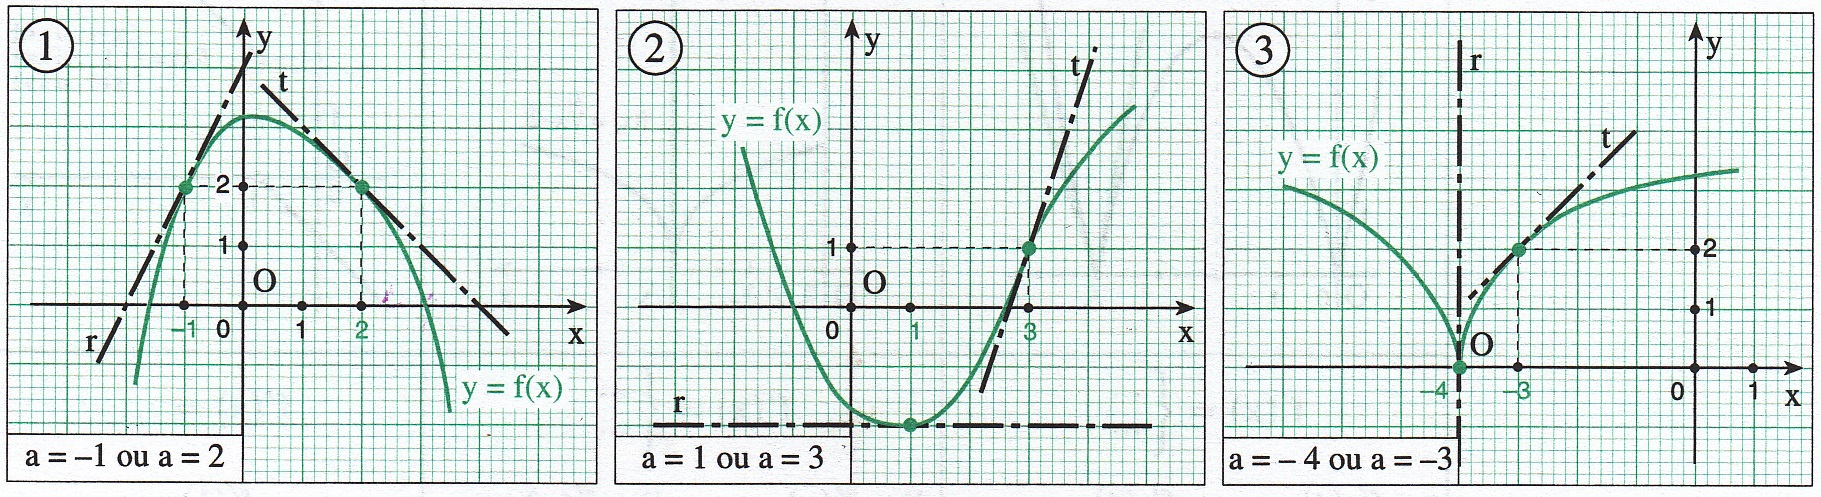
\includegraphics[height=4.5cm]{ex_10.jpg}
\end{center}
\end{exo}

%\begin{solu}
%\begin{benumerate}
%\begin{multicols}{2}
%\item[1] $f'(-1)=2$, $f'(2)=-1$
%\item[2] $f'(1)=0$, $f'(3)=3$
%\item[3] f n'est pas dérivable en $-4$, $f'(-3)=1$
%\end{multicols}
%\end{benumerate}
%\end{solu}

\begin{exo} Observe les tangentes à $G_f$ au point d'abscisse $a$, dis si la fonction $f$ est dérivable au point d'abscisse $a$. Justifie chaque fois ta réponse.
\begin{center}
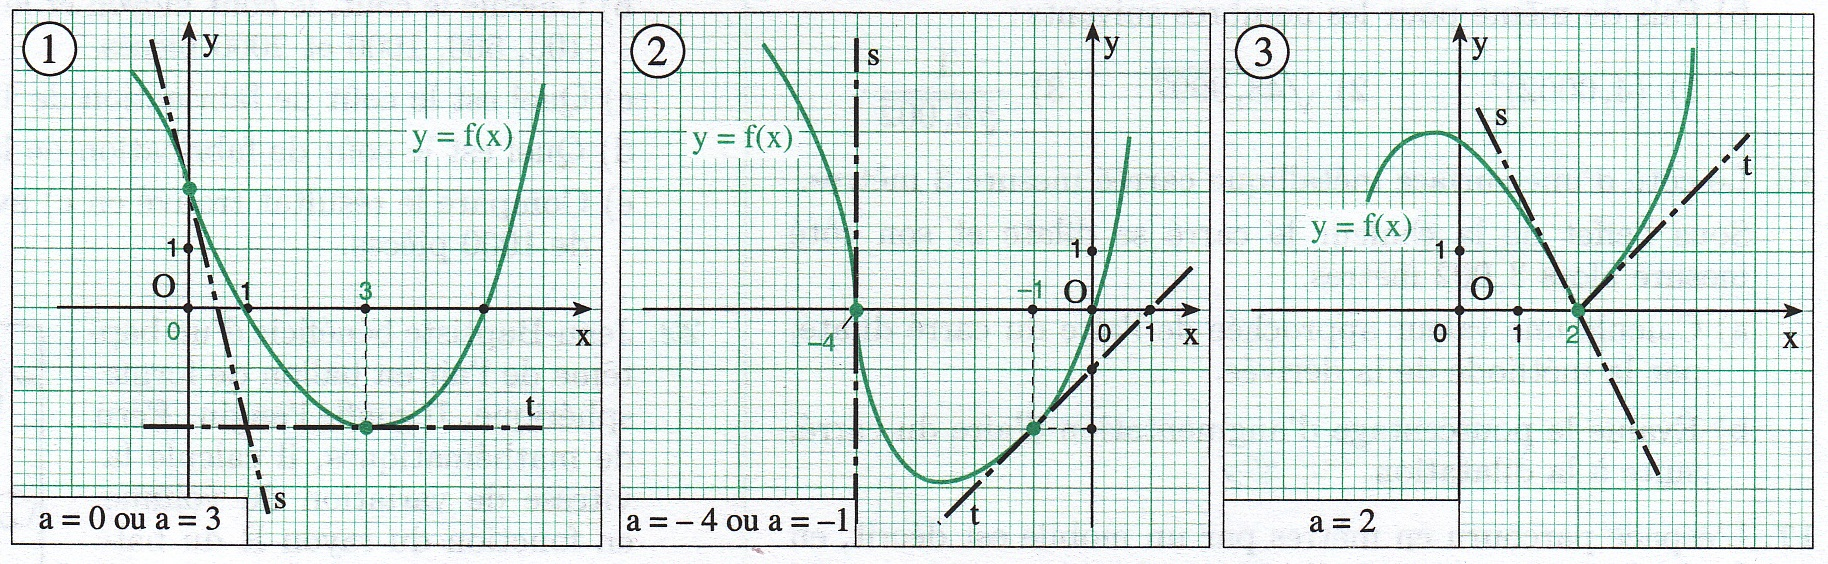
\includegraphics[height=5cm]{ex_12.jpg}
\end{center}
\end{exo}

%\begin{solu}
%\begin{benumerate}
%\begin{multicols}{2}
%\item[1] $f$ est dérivable en 0 et en 3
%\item[2] $f$ est dérivable en $-1$ mais pas en $-4$
%\item[3] $f$ n'est pas dérivable en 2
%\end{multicols}
%\end{benumerate}
%\end{solu}

\chapter{Optimisation} 
Une des applications les plus connues des fonctions dérivables est l'optimisation. Nous avons déjà abordé ce sujet avec la question de la meilleure forme à donner à un cylindre pour minimiser son aire, ce qui nous a permis de découvrir le résultat suivant :
\begin{thé} [Théorème de Fermat]
Soit $I = ]a,b[$ un intervalle. Soit $f : I \to \rr$ une fonction dérivable. \\
Si un point $c \in I$ est un point de minimum ou de maximum de $f$, alors $f'(c)=0$.
\end{thé}
Ce théorème est la base de la stratégie qui utilise les dérivées pour résoudre des problèmes d'optimisation. En effet, ce théorème a la conséquence suivante : si nous cherchons à optimiser une fonction dérivable (c'est-à-dire chercher un point de maximum ou un point de minimum d'une fonction), les seuls \og candidats \fg{} possibles\footnote{(si la fonction est définie sur un intervalle ouvert)} pour un point de maximum ou un point de minimum d'une fonction sont les points qui annulent la dérivée. Il suffit donc de chercher ces points et comparer la valeur de la fonction en ces points pour déterminer les points de maximum et les points de minimum de la fonction. \\
Néanmoins, il y a moyen de raffiner cette stratégie en établissant deux liens importants :
\begin{enumerate}
\item Le lien entre la croissance d'une fonction dérivable et le signe de sa dérivée.
\item Le lien entre la concavité d'une fonction deux fois dérivable et le signe de sa dérivée seconde.
\end{enumerate}
Nous allons découvrir ces deux liens importants\footnote{Mais nous n'aurons malheureusement pas l'occasion de les démontrer.}, puis les exploiter pour développer un \og théorème final d'optimisation \fg{} qui correspondra à une stratégie efficace destinée à résoudre toutes sortes de problèmes d'optimisation.
\begin{rema}
Malheureusement, nous n'avons pas l'occasion de démontrer le moindre des résultats de cette section dans un cours de mathématiques de $4$ heures/semaine. Nous essayerons malgré tout de donner les intuitions qui se cachent derrière chacun de ceux-ci afin qu'ils ne soient pas incompréhensibles.
\end{rema}
Avant toute autre chose, donnons quelques définitions\footnote{Certaines d'entre elles ont normalement déjà été données en quatrième année.}.
\begin{déf}
Soit $I$ un intervalle et soit $f : I \to \rr$.\\
Un nombre réel $M \in \\$ est un \emph{maximum} de $f$ s'il existe $c \in I$ tel que $f(c)=M$ et si $\forall x \in I$, $M \ge f(x)$.
\end{déf}
\begin{déf}
Soit $I$ un intervalle et soit $f : I \to \rr$.\\
Un nombre réel $m \in \\$ est un \emph{minimum} de $f$ s'il existe $c \in I$ tel que $f(c)=m$ et si $\forall x \in I$, $m \le f(x)$.
\end{déf}
\begin{déf}
Soit $I$ un intervalle et soit $f : I \to \rr$.\\
Un point $c$ est un \emph{point de maximum} de $f$ si $f(c)$ est un maximum de $f$.
\end{déf}
\begin{déf}
Soit $I$ un intervalle et soit $f : I \to \rr$.\\
Un point $c$ est un \emph{point de minimum} de $f$ si $f(c)$ est un minimum de $f$.
\end{déf}
\begin{exe}
La fonction :
\begin{align*}
f : \rr &\to \rr \\
x &\mapsto (x-1)^2 -2
\end{align*}
dont le graphe est
\begin{center}
		\begin{tikzpicture}[xmin=-5,xmax=5,ymin=-5,ymax=5,scale=0.6]{\grille\axes}
		\draw[thick] plot[domain=-1.66:3.66](\x,{(\x -1)*(\x -1)-2});
		\end{tikzpicture}
	\end{center}
a comme minimum $-2$ et a comme point de minimum $1$. Elle n'a pas de maximum (et donc pas de point de maximum).
\end{exe}
Les points où la dérivée d'une fonction dérivable s'annule sont appelés points critiques :
\begin{déf}
Soit $I=]a;b[$ un intervalle et soit $f : I \to \rr$ dérivable.\\
Un point $c \in I$ est un \emph{point critique} de $f$ si $f'(c)=0$.
\end{déf}
On peut donc reformuler le théorème de Fermat de la façon suivante :
\begin{thé} [Théorème de Fermat]
Soit $I = ]a,b[$ un intervalle. Soit $f : I \to \rr$ une fonction dérivable. \\
Si un point $c \in I$ est un point de minimum ou de maximum de $f$, alors $c$ est un point critique de $f$.
\end{thé}
La réciproque de ce théorème est-elle valide ? Malheureusement, non, il existe toutes sortes de points critiques :
\begin{itemize}
\item [$\bullet$] Les points de maximum et de minimum, ce sont les points critiques qui nous intéressent lorsqu'on essaye de résoudre un problème d'optimisation. \\
Par exemple, pour la fonction dont la graphe est le suivant :
\begin{center}
		\begin{tikzpicture}[xmin=-5,xmax=5,ymin=-5,ymax=5,scale=0.6]{\grille\axes}
		\draw[thick] plot[domain=-4.45:0.45](\x,{-(\x +2)*(\x +2)+1});
		\end{tikzpicture}
	\end{center}
Le point $-2$ est l'unique point critique de la fonction et c'est un point de maximum de la fonction.
\item [$\bullet$] Les points de maximum et de minimum locaux, que nous n'étudierons pas en détail dans le cadre de ce cours. \\
Par exemple, pour la fonction dont la graphe est le suivant :
\begin{center}
		\begin{tikzpicture}[xmin=-5,xmax=5,ymin=-5,ymax=5,scale=0.6]{\grille\axes}
		\draw[thick] plot[domain=-2.28:2.28,samples=100](\x,{-(\x +2)*(\x +1)*(\x -1)*(\x -2)});
		\end{tikzpicture}
	\end{center}
Le point $0$ est un point critique mais ce n'est pas un point de maximum ni de minimum. C'est un point de minimum local de la fonction (\og aux alentours de $0$ \fg{}, $0$ est un point de minimum de $f$, mais pas globalement).
\item [$\bullet$] Des points qui ne sont même pas des points de maximum ou de minimum local, comme par exemple les points d'inflexion, que nous définirons un peu plus loin. Ces points peuvent être très ennuyeux si on souhaite utiliser le théorème de Fermat pour optimiser une fonction.\\
Par exemple, pour la fonction dont la graphe est le suivant :
\begin{center}
		\begin{tikzpicture}[xmin=-5,xmax=5,ymin=-5,ymax=5,scale=0.6]{\grille\axes}
		\draw[thick] plot[domain=0.41:3.82,samples=100](\x,{(\x -2)*(\x -2)*(\x -2)-1});
		\end{tikzpicture}
	\end{center}
Le point $2$ est un point critique mais ce n'est pas un point de maximum ni de minimum et ce n'est même pas un point de maximum local ou un point de minimum local. C'est un point d'inflexion de ma fonction (intuitivement : la concavité de la fonction change en ce point).
\end{itemize}
Il va falloir apprendre à faire le tri parmi tous ces différents types de points critiques afin de ne garder que ceux qui nous intéressent pour un problème d'optimisation, c'est-à-dire les points de maximum et de minimum. Les deux sections qui suivent vont nous permettre de réaliser ce tri.
\section{Le lien entre la croissance d'une fonction dérivable et le signe de sa dérivée}
Commençons avec la proposition suivante :
\begin{pro} \label{dercroi}
Soit $I=]a;b[$ un intervalle et soit $f : I \to \rr$ dérivable.\\
Alors $f$ est croissante si et seulement si $\forall x \in I$, $f'(x) \ge 0$.
\end{pro}
Maintenant que nous avons une interprétation géométrique de la dérivée, la proposition \ref{dercroi} ne devrait pas vous surprendre : si une fonction est croissante, les pentes des tangentes à son graphe ne peuvent qu'être positive et inversément. \\
\begin{rema}
De la même manière, on a une proposition équivalente à la proposition \ref{dercroi} pour la décroissance : il suffit d'inverser le sens de l'inégalité.
\end{rema}
On a une proposition similaire pour la croissance stricte. Malheureusement, il n'y a alors plus équivalence, seulement implication :
\begin{pro} \label{dercroistrict}
Soit $I=]a;b[$ un intervalle et soit $f : I \to \rr$ dérivable.\\
Si $\forall x \in I$, $f'(x) > 0$, alors $f$ est strictement croissante.
\end{pro}
L'idée intuitive qui se cache dérrière cette proposition est la même que celle pour la proposition \ref{dercroi}.
\begin{rema}
À nouveau, on a de la même manière une proposition équivalente à la proposition \ref{dercroi} pour la décroissance : il suffit d'inverser le sens de l'inégalité stricte.
\end{rema}
\begin{exe}
La fonction carrée
\begin{align*}
f : \rr &\to \rr \\
x &\mapsto x^2
\end{align*}
est décroissante sur $]-\infty;0[$ et croissante sur $]0:\infty[$. Sa fonction dérivée :
\begin{align*}
f' : \rr &\to \rr \\
x &\mapsto 2x
\end{align*}
est bien négative sur $]-\infty;0[$ et positive sur $]0:\infty[$.
\end{exe}
\section{Le lien entre la concavité d'une fonction deux fois dérivable et le signe de sa dérivée seconde}
Vous avez déjà rencontré la notion de concavité dans le cas des paraboles en quatrième année, mais il est possible de généraliser cette notion. Intuitivement, l'idée est de définir une fonction convexe comme une fonction dont le graphe entre deux abscisses choisies arbitrairement se situe en dessous du graphe de la droite reliant les deux points du graphe de la fonction dont les abscisses sont celles choisies :
\begin{déf}
Soit $I$ un intervalle et soit $f : I \to \rr$.\\
Si $\forall a,b \in I$, on a $\forall x \in [a;b]$ que $f(x) \le \frac{f(b)-f(a)}{b-a}x - \frac{f(b)-f(a)}{b-a}b + f(b)$, on dit que la fonction est \emph{convexe}.
\end{déf}
\begin{déf}
Soit $I$ un intervalle et soit $f : I \to \rr$.\\
Si $\forall a,b \in I$, on a $\forall x \in [a;b]$ que $f(x) \ge \frac{f(b)-f(a)}{b-a}x - \frac{f(b)-f(a)}{b-a}b + f(b)$, on dit que la fonction est \emph{concave}.
\end{déf}
\begin{exe}
La fonction carrée est convexe tandis que la fonction racine carrée est concave.
\end{exe}
On peut alors proprement énoncer le lien annoncé entre la concavité d'une fonction deux fois dérivable et le signe de sa dérivée seconde :
\begin{pro} \label{derconv}
Soit $I=]a;b[$ un intervalle et soit $f : I \to \rr$ deux fois dérivable.\\
Si $\forall x \in I$, $f''(x) > 0$, alors $f$ est convexe.
\end{pro}
L'intuition derrière la proposition \ref{derconv} est un peu plus complexe que celle de la proposition \ref{dercroi}. Si une fonction $f$ deux fois dérivable et définie sur un intervalle a sa dérivée seconde qui est strictement positive, cela implique par la proposition \ref{dercroistrict} que $f'$ est strictement croissante, autrement dit que les pentes des tangentes deviennent de plus en plus grandes au fur et à mesure que les abscisses augmentent. Dès lors, le graphe de la fonction est d'une certaine manière \og bercé \fg{} par ses tangentes par en dessous, celui-ci est donc nécessairement \og tourné vers le haut \fg{}, ce que nous pouvons à présent exprimer plus clairement : la fonction est convexe.
\begin{rema}
On a une proposition équivalente à la proposition \ref{derconv} pour la concavité : il suffit d'inverser le sens de l'inégalité stricte de l'hypothèse.
\end{rema}
\begin{exe}
La fonction carrée
\begin{align*}
f : \rr &\to \rr \\
x &\mapsto x^2
\end{align*}
est convexe. Sa dérivée seconde :
\begin{align*}
f'' : \rr &\to \rr \\
x &\mapsto 2
\end{align*}
est bien strictement positive.
\end{exe}
\section{Un théorème d'optimisation}
Nous avons à présent tout ce qu'il nous faut pour développer un théorème final d'optimisation\footnote{Il est à noter que celui-ci est assez artificiel, est construit sur mesure pour ce cours et est finalement assez limité. Il est possible de le généraliser très facilement.}. Celui-ci nous permettra non seulement de nous assurer qu'un problème d'optimisation possède une solution, mais aussi de trouver les solutions potentielles et de faire le tri parmi celles-ci. \\
Ce théorème est présenté d'une façon peu orthodoxe mais qui permet de faire ressortir une stratégie pour résoudre les problèmes d'optimisation proposés dans le syllabus d'exercices annexe, tout en en l'expliquant au fur et à mesure de son développement.
\begin{thé} [Théorème final d'optimisation : maximisation]
Soit $I=[a;b]$ un intervalle et soit $f : I \to \rr$ continue et deux fois dérivable sur $]a;b[$ avec $f'$ et $f''$ continue.\\
Nous souhaitons trouver un point de maximum pour $f$. Notons tout d'abord que le théorème des bornes atteintes nous assure que celui-ci existe. \\
Ensuite, supposons que $a$ et $b$ ne sont pas des points de maximum (si un des deux est un point de maximum, maximiser la fonction est immédiat). \\
Dès lors, tout point $c \in I$ qui est un point de maximum appartient à $]a;b[$ et donc, par le théorème de Fermat, $c$ est un point critique. \\
Alors, si $c$ est le seul point critique qui vérifie une des deux conditions suivantes :
\begin{enumerate}
\item On a pour le tableau de signe de $f'$ :
\begin{tabular}{|c|c c c|}
  \hline
  x & ~~~~ & c & ~~~~ \\
  \hline
  f'(x) & + & 0 & - \\
  \hline
\end{tabular}
~~\\
~~\\
Autrement dit : si $c$ est le seul point critique pour lequel la dérivée est négative avant $c$ et positive après $c$, ce qui implique par la proposition \ref{dercroi} et son équivalent pour la décroissance que $f$ est croissante avant $c$ et décroissante après $c$ (et donc, intuitivement : $c$ est donc un \og sommet \fg{}, c'est-à-dire un maximum local).
\item On a $f''(c) < 0$. \\
Autrement dit : si $c$ est le seul point critique où la dérivée seconde est strictement négative, ce qui implique par l'équivalent pour la décroissance stricte de la proposition \ref{dercroistrict} que $f'$ est strictement décroissante au voisinage de $c$ et donc que $f$ est concave sur un voisinage de $c$ (et donc, intuitivement : $c$ est donc un \og sommet \fg{}, c'est-à-dire un maximum local).
\end{enumerate}
Alors $c$ est le point de maximum de $f$ (puisque nous sommes certains qu'il existe un tel point de maximum et que le point $c$ est le seul candidat possible, ça ne peut être que lui).
\end{thé}
De la même façon, on a pour la recherche d'un point de minimum :
\begin{thé} \label{tfomin} [Théorème final d'optimisation : minimisation]
Soit $I=[a;b]$ un intervalle et soit $f : I \to \rr$ continue et deux fois dérivable sur $]a;b[$ avec $f'$ et $f''$ continue.\\
Nous souhaitons trouver un point de minimum pour $f$. Notons tout d'abord que le théorème des bornes atteintes nous assure que celui-ci existe. \\
Ensuite, supposons que $a$ et $b$ ne sont pas des points de minimum (si un des deux est un point de minimum, minimiser la fonction est immédiat). \\
Dès lors, tout point $c \in I$ qui est un point de minimum appartient à $]a;b[$ et donc, par le théorème de Fermat, $c$ est un point critique. \\
Alors, si $c$ est le seul point critique qui vérifie une des deux conditions suivantes :
\begin{enumerate}
\item On a pour le tableau de signe de $f'$ :
\begin{tabular}{|c|c c c|}
  \hline
  x & ~~~~ & c & ~~~~ \\
  \hline
  f'(x) & - & 0 & + \\
  \hline
\end{tabular}
~~\\
~~\\
Autrement dit : si $c$ est le seul point critique pour lequel la dérivée est positive avant $c$ et négative après $c$, ce qui implique par la proposition \ref{dercroi} et son équivalent pour la décroissance que $f$ est décroissante avant $c$ et croissante après $c$ (et donc, intuitivement : $c$ est donc un \og le fond d'une vallée \fg{}, c'est-à-dire un minimum local).
\item On a $f''(c) > 0$. \\
Autrement dit : si $c$ est le seul point critique où la dérivée seconde est strictement positive, ce qui implique par la proposition \ref{dercroistrict} que $f'$ est strictement croissante au voisinage de $c$ et donc que $f$ est convexe sur un voisinage de $c$ (et donc, intuitivement : $c$ est donc un \og le fond d'une vallée \fg{}, c'est-à-dire un minimum local).
\end{enumerate}
Alors $c$ est le point de minimum de $f$ (puisque nous sommes certains qu'il existe un tel point de minimum et que le point $c$ est le seul candidat possible, ça ne peut être que lui).
\end{thé}
\begin{exe}
Vérifions la validité du théorème \ref{tfomin} sur notre problème d'optimisation de l'introduction. Le point $c = \sqrt[3]{\frac{660}{4 \pi}}$ était l'unique point critique de la fonction (éventuellement réduite sur $[1;10]$) et était l'unique point de minimum de la fonction. Vérifions que les conditions données par le théorème \ref{tfomin} étaient justement toutes les deux respectées. \\
Rappelons que nous avions pour tout $x \in ]0;\infty[$ :
$$A'(x) = 4\pi x - \frac{660}{{x}^2}$$
On a donc bien :
\begin{center}
\begin{tabular}{|c|c c c|}
  \hline
  x & ~~~~ & $\sqrt[3]{\frac{660}{4 \pi}}$ & ~~~~ \\
  \hline
  f'(x) & - & 0 & + \\
  \hline
\end{tabular}
\end{center}
~~\\
De plus, $A$ est deux fois dérivable et pour tout $x \in ]0;\infty[$ :
$$A''(x) = 4\pi + \frac{1320}{{x}^3}$$
Et on a bien :
$$A''(\sqrt[3]{\frac{660}{4 \pi}}) = 12\pi >0$$
Le théorème est donc bien cohérent avec ce que nous avions déjà annoncé et nous aurait permis de découvrir directement la solution que nous avions trouvée.
\end{exe}
Il est temps d'appliquer nos théorèmes finaux d'optimisation sur de nombreux autres exemples. Heureusement, les exercices de problèmes d'optimisation ne manquent pas !
\begin{exo*}
Voir dossier annexe.
\end{exo*}

\chapter{Résultats importants sur les fonctions dérivables (optionnel)}

Dans cette section, attardons-nous un instant sur deux résultats importants qui concernent les fonctions dérivables. \\
Tout d'abord, est-il possible de faire un lien entre la notion de dérivabilité et celle de continuité ? Cette question est d'autant plus légitime puisque jusqu'ici, toutes les fonctions dérivables que nous avons utilisées et que nous connaissons sont continues. Ce n'est pas un hasard, car nous pouvons démontrer facilement la proposition suivante :
\begin{pro} \label{dercont}
Soit $I=]a;b[$ un intervalle et soit $f:I\to \rr$ dérivable en un point $c \in I$.\\
Alors $f$ est continue en $c$.
\end{pro}
\begin{proof}
Montrer que $f$ est continue en $c$ revient à montrer que $\lim_{x \to c} f(x)=f(c)$ (voir chapitre sur les fonctions continues), ce qui revient à montrer que $\lim_{x \to c} f(x)-f(c)=0$ (puisque $f(c)$ est une constante).\\
Or, nous savons que $\lim_{x \to c} \frac{f(x)-f(c)}{x-c} = f'(c)$ (puisque $f$ est dérivable en $c$) et que $\lim_{x \to c} (x-c)=0$.\\ Dès lors, par les propriétés des limites :
$$\lim_{x \to c} f(x)-f(c) = \lim_{x \to c} \frac{f(x)-f(c)}{x-c} . (x-c)=\lim_{x \to c} \frac{f(x)-f(c)}{x-c} . \lim_{x \to c} (x-c)= f'(c).0=0$$
\end{proof}
Toutes les fonctions dérivables sont donc automatiquement continues.\\
~~\\
Après la proposition \ref{dercont}, parlons du résultat peut-être le plus important sur les fonctions dérivables : le théorème des accroissements finis.
\begin{thé} Théorème des accroissements finis]
Soit $I=[a;b]$ un intervalle et soit $f:I\to \rr$ dérivable sur $]a;b[$ et continue en $a$ et $b$.
Alors il existe $c \in ]a;b[$ tel que $f(b)-f(a)=f'(c)(b-a)$.
\end{thé}
Malheuresement, ce théorème est relativement difficile à démontrer. Heureusement, il possède une interprétation géométrique qui le rend assez intuitif. En effet, en divisant les deux membres de l'égalité $f(b)-f(a)=f'(c)(b-a)$ dans la conclusion du théorème, on obtient l'égalité $\frac{f(b)-f(a)}{b-a}=f'(c)$. Essentiellement, le théorème nous dit donc que nous pouvons être certains qu'il y a un point $c$ entre $a$ et $b$ tel que la pente de la tangente au graphe de $f$ au point d'abscisse $c$ sera identique à la pente de la droite joignant les points $(a;f(a))$ et $(b;f(b))$. \\
Un exemple concret de cette interprétation géométrique du théorème serait le suivant : si la distance entre l'école et maison est de $1000$m et si l'école est à une altitude plus élevée de $100$m que celle de ma maison, je peux être certain qu'il y aura un moment dans mon trajet depuis chez moi jusqu'à l'école où la pente de la route (l'inclinaison du sol) sera de $10$\% (à condition que je n'emprunte pas d'escalier et que je n'utilise pas d'ascenseur). \\
Le théorème des accroissements finis possède énormément d'applications en mathématiques. Par exemple, il permet de démontrer que les seules fonctions dérivables définies sur un intervalle dont la dérivée est nulle sont les fonctions constantes :
\begin{pro}
Soit $I=[a;b]$ un intervalle et soit $f:I\to \rr$ dérivable sur $]a;b[$ et continue en $a$ et $b$, telle que $\forall x \in ]a;b[$, $f'(x)=0$.
\end{pro}
\begin{proof}
Montrons que $\forall x \in [a;b]$, $f(x)=f(a)$. \\
Soit $x \in [a;b]$. Si $x =a$, on a évidemment $f(x)=f(a)$. \\
Si $x \neq a$, alors par le théorème des accroissements finis appliqué à la fonction $f_{|[a;x]}$, on est certain qu'il existe $x \in ]a;x[$ tel que $f(x)-f(a)=f'(c)(x-a)$. Or, par hypothèse, on sait que $f'(c)=0$, donc on en déduit que $f(x)-f(a)=0$, c'est-à-dire que $f(x)=f(a)$.
\end{proof}
Nous n'utiliserons pas cette proposition cette année, mais elle sera cruciale l'année prochaine pour la démonstration du théorème fondamental du calcul différentiel et intégral\footnote{Ne l'oubliez donc pas !}.\\
~~\\
Il y aurait encore beaucoup à dire sur les dérivées, mais nous allons devoir nous arrêter là. Néanmoins, les dérivées reviendront en force l'année prochaine, lorsque vous aborderez le sujet passionant des intégrales.

\chapter{Annexe}

Dans cette section facultative, nous allons démontrer les deux propositions suivantes :

\begin{pro*}
	Soit $g : \rr \to \rr$ dérivable. \\
Alors $g$ est continue.
\end{pro*}
\begin{pro*}
	Soient deux fonctions $f : \rr \to \rr$ et $g : \rr \to \rr$ dérivables. \\
Alors $f \circ g : \rr \to \rr$ est dérivable et pour tout $x \in \rr$ on a :
$$(f \circ g)'(x) = (f' \circ g)(x).g'(x)$$
\end{pro*}

Commençons par démontrer la plus facile des deux :
\begin{pro} \label{derdonccont}
	Soit $g : \rr \to \rr$ dérivable. \\
Alors $g$ est continue.
\end{pro}
\begin{proof}
Fixons $a \in \rr$ et montrons que $g$ est continue en $a$. \\
Pour tout $x \neq a$ :
$$g(x)-g(a)=\frac{g(x) - g(a)}{x-a}.(x-a)$$
Puisque $g$ est dérivable en $a$ on sait que :
$$\lim\limits_{x \to a} \frac{g(x) - g(a)}{x-a} = g'(a)$$
De plus, on a :
$$\lim\limits_{x \to a} (x-a)=0$$
En conclusion, par les propriétés des limites :
$$\lim\limits_{x \to a} g(x)-g(a)=\lim\limits_{x \to a} \frac{g(x) - g(a)}{x-a}.(x-a) = \lim\limits_{x \to a}\frac{g(x) - g(a)}{x-a} . \lim\limits_{x \to a}(x-a)=g'(a).0=0$$
Puisque $\lim\limits_{x \to a} g(x)-g(a)=0$, on a $\lim\limits_{x \to a} g(x)=\lim\limits_{x \to a} g(a)=g(a)$. Par le théorème reliant fonctions continues et limites (voir théorème 4.0.6 du chapitre 3), $g$ est donc continue en $a$.
\end{proof}

À présent, passons à la deuxième :

\begin{pro}
	Soient deux fonctions $f : \rr \to \rr$ et $g : \rr \to \rr$ dérivables. \\
Alors $f \circ g : \rr \to \rr$ est dérivable et pour tout $x \in \rr$ on a :
$$(f \circ g)'(x) = (f' \circ g)(x).g'(x)$$
\end{pro}
\begin{proof}
Nous devons donc montrer que pour tout $a \in \rr$, la limite :
$$\lim\limits_{x \to a} \frac{f(g(x)) - f(g(a))}{x-a}$$
existe et est égale à :
$$f'(g(a)).g'(a)$$
Si $a$ est le seul point où la fonction $g$ vaut $g(a)$, la démonstration est facile. En effet, on a alors pour tout $x \neq a$ :
$$\frac{f(g(x)) - f(g(a))}{x-a} = \frac{f(g(x)) - f(g(a))}{g(x)-g(a)} . \frac{g(x) - g(a)}{x-a}$$
Et donc, comme $\lim\limits_{x \to a} \frac{g(x) - g(a)}{x-a} = g'(a)$ (car $g$ est dérivable en $a$) et $\lim\limits_{x \to a} \frac{f(g(x)) - f(g(a))}{g(x)-g(a)} = f'(g(a))$ (car $f$ est dérivable en $g(a)$), on a par les propriétés des limites :
$$\lim\limits_{x \to a} \frac{f(g(x)) - f(g(a))}{x-a} =\lim\limits_{x \to a} \frac{f(g(x)) - f(g(a))}{g(x)-g(a)} = f'(g(a)) .\lim\limits_{x \to a} \frac{g(x) - g(a)}{x-a}=f'(g(a)).g'(a)$$
Malheureusement, on ne peut pas être certain que $a$ est le seul point où la fonction $g$ vaut $g(a)$ et donc qu'on ne divise pas par $0$ en considérant l'expression $\frac{f(g(x)) - f(g(a))}{g(x)-g(a)}$. Il faut donc ruser. Nous allons utiliser la théorie des fonctions continues. \\
Fixons $a \in \rr$. Par le théorème reliant fonctions continues et limites (voir théorème 4.0.6 du chapitre 3), dire que $f$ est dérivable en $g(a)$ est équivalent au fait que la fonction suivante est continue en $g(a)$ :
\begin{align*}
h : \rr \to& \rr \\
x \mapsto& \begin{cases}
\frac{f(x) - f(g(a))}{x-g(a)} & \text{si } x \neq g(a) \\
f'(g(a)) & \text{si } x = g(a)
\end{cases}
\end{align*}
Or, pour tout $x \neq a$, on a\footnote{Même si $g(x)=g(a)$ ! Si $g(x)=g(a)$, le membre de gauche s'annule mais le membre de droite aussi.} :
$$\frac{f(g(x)) - f(g(a))}{x-a} = h(g(x)) . \frac{g(x) - g(a)}{x-a}$$
Puisque $h$ est continue en $g(a)$ et que $g$ est dérivable et donc continue (voir proposition \ref{derdonccont} ci-dessus) en $a$ (ce qui implique par le théorème 4.0.6 du chapitre 3 que $\lim\limits_{x \to a}g(x)-g(a)$), par le théorème théorème 4.0.8 du chapitre 3 :
$$\lim\limits_{x \to a} h(g(x))=h(g(a))$$
Puisque $g$ est dérivable en $a$ :
$$\lim\limits_{x \to a} \frac{g(x) - g(a)}{x-a} =g'(a)$$
Donc, par les propriétés des limites :
\begin{align*}
\lim\limits_{x \to a}\frac{f(g(x)) - f(g(a))}{x-a} &= \lim\limits_{x \to a}  h(g(x)) . \frac{g(x) - g(a)}{x-a} \\
&= \lim\limits_{x \to a}  h(g(x)) . \lim\limits_{x \to a} \frac{g(x) - g(a)}{x-a} \\
&= h(g(a)).g'(a)=f'(g(a)).g'(a)
\end{align*}
Ce qui est justement ce qu'on voulait démontrer.
\end{proof}
\end{document}
